\documentclass{fisatprojectfinal}
\usepackage{listings}

\lstset{
    breaklines=true,                    % sets automatic line breaking
%   breakatwhitespace=false,            % sets if automatic breaks should only happen at whitespace
    prebreak = \raisebox{0ex}[0ex][0ex]{\ensuremath{\hookleftarrow}} % just as an example
}

\title{Pose Estimation Using Deep Learning}
\team{Aman K. Shihab \\ Aneeta Shajan}
\author{Aman K. Shihab}
\regno{FIT19CS015}
\begin{document}
\maketitle
\makecert

\newpage
\pagenumbering{roman}
\setcounter{page}{1}
\newgeometry{top=4cm,bottom=0.1cm}
\thispagestyle{plain}
\renewcommand\abstractname{ABSTRACT}
\begin{abstract}
\vspace{5cm}
Single-person human pose estimation facilitates markerless movement analysis in sports, as well as in clinical applications.
Still, state-of-the-art models for human pose estimation generally do not meet the requirements of real-life applications.
The proliferation of deep learning techniques has resulted in the development of many advanced approaches. However,
with the progresses in the field, more complex and inefficient models have also been introduced, which have caused
tremendous increases in computational demands. To cope with these complexity and inefficiency challenges, we propose
a novel convolutional neural network architecture, called EfficientPose, which exploits recently proposed EfficientNets
in order to deliver efficient and scalable single-person pose estimation. EfficientPose is a family of models harnessing
an effective multi-scale feature extractor and computationally efficient detection blocks using mobile inverted bottleneck
convolutions, while at the same time ensuring that the precision of the pose configurations is still improved. Due to its low
complexity and efficiency, EfficientPose enables real-world applications on edge devices by limiting the memory footprint
and computational cost. The results from our experiments, using the challenging MPII single-person benchmark, show that
the proposed EfficientPose models substantially outperform the widely-used OpenPose model both in terms of accuracy and
computational efficiency. In particular, our top-performing model achieves state-of-the-art accuracy on single-person MPII,
with low-complexity ConvNets. The architecture was finetuned on the Leeds Sports dataset and some improvement in accuracy was obtained.
\end{abstract}



\newpage
\renewcommand\abstractname{Contribution by Author}
\thispagestyle{plain}
\begin{abstract}
\vspace{5cm}
The model was fine-tuned using the Leeds Sports dataset. We observed some points increase in accuracy of the model.
Work is progressing currently on obtaining dataset to fine tune it for Physiotherapy pose detection and correction.
\vspace{1cm}
\begin{flushright}
Aman K. Shihab
\end{flushright}
\end{abstract}

\newpage
\renewcommand\abstractname{ACKNOWLEDGEMENT}
\thispagestyle{plain}
\begin{abstract}
\vspace{5cm}
It gives me a great sense of pleasure to present the report of the project work undertaken during BTech 
semester 6. I owe a special debt of gratitude to my Project Mentor \textbf{Mr. Pankaj Kumar G} for guiding and supporting us
throughout the course of this project. It is only due to his trust and support we were able to complete this project successfully. I would also like to acknowledge
\textbf{Cognitive Computing Research Centre (CCRC) FISAT} for providing us with an environment and the experience to conduct research projects.
\par
I would like to extend my gratitude to our project co-ordinators \textbf{Ms. Chethna Joy} and \textbf{Ms. Remya R} for helping us in 
keeping the course of our project in track providing with appropriate ideas and information which were useful during the duration of our project work.
\par
Finally, my deepest thanks to \textbf{Computer Science and Engineering Deptartment, FISAT} and our HOD \textbf{Dr. Jyothish K. John} for providing us with the
correct environment and opprotunities to learn and grow. I would like to thank our university, for including this project as a part of the degree program.
\vspace{1cm}
\begin{flushright}
Aman K. Shihab
\end{flushright}
\end{abstract}
\newpage

\restoregeometry
\tableofcontents
\thispagestyle{plain}
\newpage

\cleardoublepage
\addcontentsline{toc}{chapter}{\listfigurename}
\listoffigures
\newpage

% \cleardoublepage
% \addcontentsline{toc}{chapter}{List Of Tables}
% \listoftables
% \newpage



\chapter{Introduction}
\pagenumbering{arabic}
\setcounter{page}{1}
\renewcommand{\baselinestretch}{1.50}
\section{Overview}
Single-person human pose estimation (HPE) refers to the
computer vision task of localizing human skeletal keypoints
of a person from an image or video frames. Single-
person HPE has many real-world applications, ranging from
outdoor activity recognition and computer animation to clinical assessments of motor repertoire and skill practice
among professional athletes. The proliferation of deep
convolutional neural networks (ConvNets) has advanced
HPE and further widen its application areas. ConvNet-based
HPE with its increasingly complex network structures,
combined with transfer learning, is a very challenging task.
However, the availability of high-performing ImageNet
backbones, together with large tailor-made datasets, such
as MPII for 2D pose estimation, has facilitated the
development of new improved methods to address the
challenges.
\begin{figure}[h!]
\begin{center}
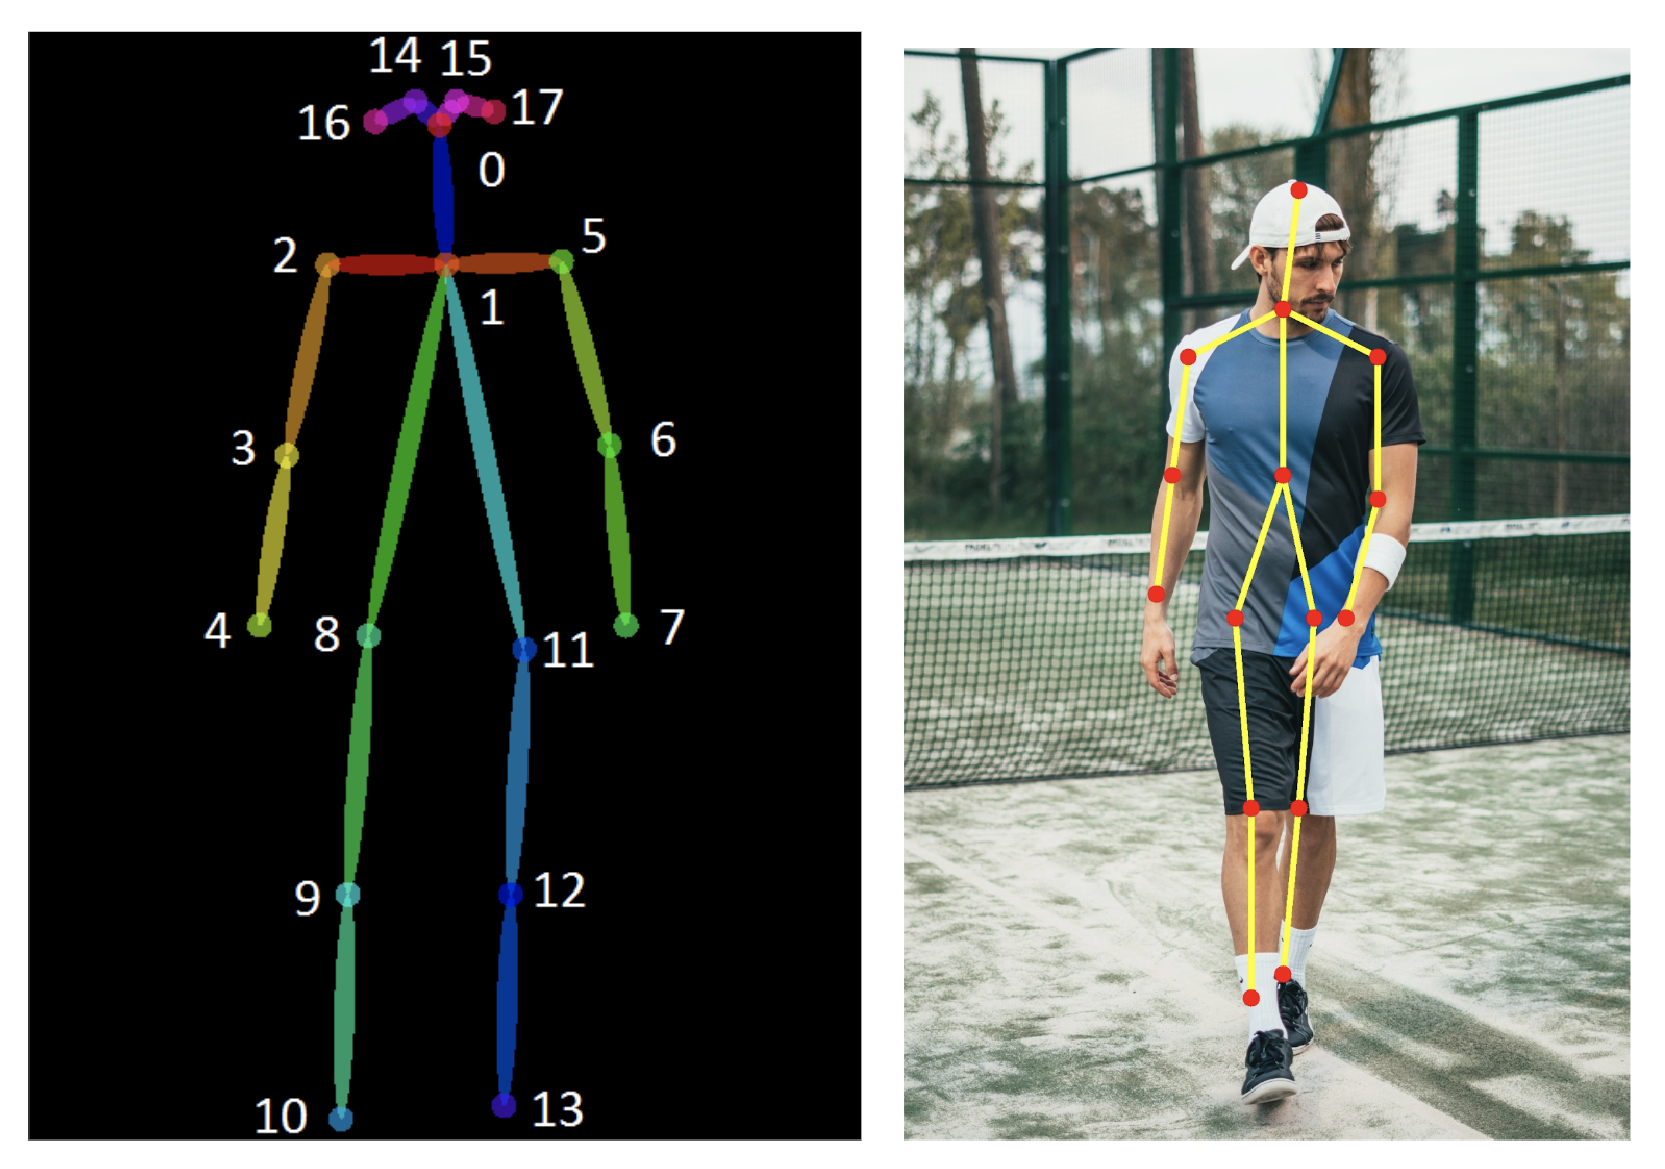
\includegraphics[scale=.3]{pose-estimation}
\caption{Human Pose Estimation Demo}
\end{center}
\end{figure}
An increasing trend in computer vision has driven towards
more efficient models. Recently, Efficient-
Net was released as a scalable ConvNet architecture,
setting benchmark record on ImageNet with a more com-
putationally efficient architecture. 
\section{Problem Statement}

Despite the availability of more performant, efficient layers and architectures, it has not quite translated
into fruitful results within human pose estimation. There is still a lack of architectures that
are both accurate and computationally efficient at the same
time. In general, current state-of-the-art architectures are
computationally expensive and highly complex, thus making them hard to replicate, cumbersome to optimize, and
impractical to embed into real-world applications. \par

Minimal and efficient model architectures are coveted for their ability to run on edge devices with minimal hardware requirements.
This also greatly reduces the response times thereby becoming increasingly relevant for real-time applications.
The ability to run real-time is a crucial feature for pose estimation, because often times in most applications it is desirable to obtain the outputs instantly to judge the output.

\section{Objective}

Primary objective is to exploit recent advances in ConvNets and shed some light onto
an improved approach called EfficientPose. The main idea
is to modify OpenPose, a well-known pose estimation model into a family of scalable ConvNets
for high-precision and computationally efficient single-person
pose estimation from 2D images. 
Then we evaluate the EfficientPose model by comparing
it against the original OpenPose model on single-person
HPE. After that, we compare it against the current state-of-
the-art single-person HPE methods on the official MPII
challenge, focusing on accuracy as a function of the number
of parameters. EfficientPose models aim to
elicit high computational efficiency, while bridging the gap
in availability of high-precision HPE networks.

\chapter{Related works}

Ever since the increased adoption of ConvNets for HPE following the
success of DeepPose has set the path for accurate HPE.
Another breakthrough in HPE was provided by OpenPose. OpenPose comprises a multi-
stage architecture performing a series of detection passes.
Provided an input image of 368 × 368 pixels, OpenPose
utilizes an ImageNet pretrained VGG-19 backbone to
extract basic features. The features are
supplied to a DenseNet-inspired detection block
arranged as five dense blocks, each containing three 3×
3 convolutions with PReLU activations. The detection
blocks are stacked in a sequence. First, four passes of part affinity fields map the associations
between body keypoints. Subsequently, two detection
passes predict keypoint heatmaps to
obtain refined keypoint coordinate estimates. In terms of
level of detail in the keypoint coordinates, OpenPose is
restricted by its output resolution of 46 × 46 pixels.
The OpenPose architecture can be improved by recent
advancements in ConvNets, as follows: First, automated
network architecture search has found backbones that are more precise and efficient in image
classification than VGG and ResNets. Compound model scaling can
balance the image resolution, width (number of networkchannels), and depth (number of network layers). This
resulted in scalable convolutional neural networks, called
EfficientNets, with which the main goal was to provide
lightweight models with a sensible trade-off between model
complexity and accuracy across various computational
budgets. For each model variant EfficientNet, from the
most computationally efficient one being EfficientNet-B0
to the most accurate model, EfficientNet-B7.The total no. of FLOPS increases by a factor of 2, given by:
	
	$$
	(\alpha. \beta^2. \gamma ^ 2) ^ \phi
	$$
where $$ \alpha = 1.2 , \beta = 1.1, \gamma = 1.15 $$
They denote the coefficients for depth, width and resolution respectively.
% \begin{table}[h!]
% \begin{center}
% 	\caption{World Population Table} 
% \begin{tabular}{|c|c|c|c|}
	
% \hline Rank & Country & Population  & Percentage  \\ 
% \hline 1 & China & 1,347,350,000 & 19.24\% \\ 
% \hline 2 & India & 1,210,193,422  & 17.28\% \\ 
% \hline 3 & United States & 313,269,000 & 4.47\% \\ 
% \hline 
% \end{tabular}
% %\caption{World Population Table} 
% \end{center}
% \end{table}
\begin{figure}[h!]
	\begin{center}
	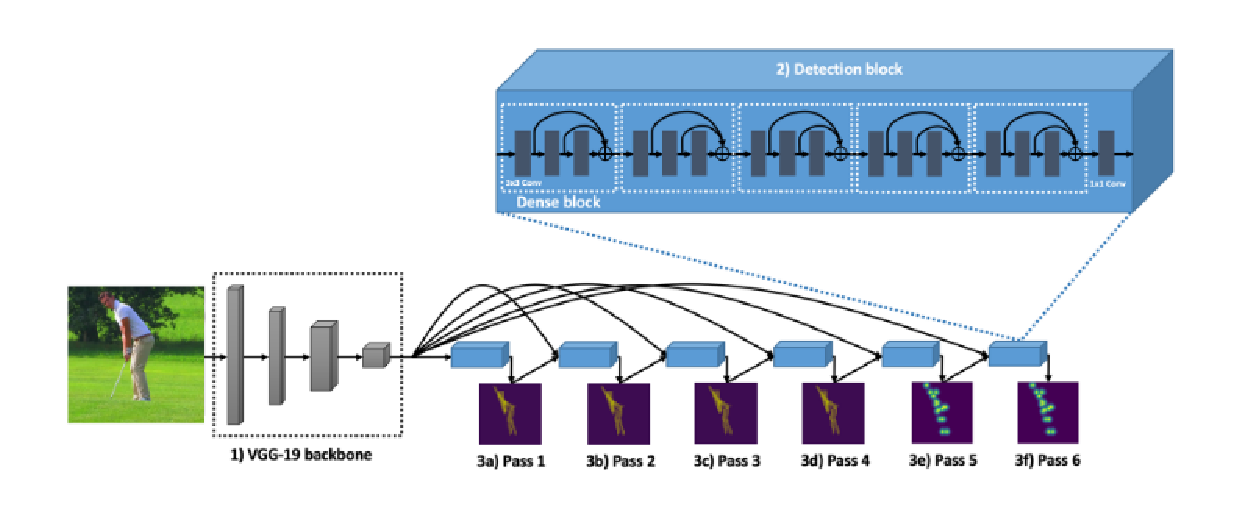
\includegraphics[scale=.8]{OpenPose}
	\caption{OpenPose}
	\end{center}
	\end{figure}
\par
Second, parallel multi-scale feature extraction has improved
the precision levels in HPE, emphasizing
both high spatial resolution and low-scale semantics.
However, existing multi-scale approaches in HPE are
computationally expensive, both due to their large size and
high computational requirements. For example, a typical
multi-scale HPE approach has often a size of 16 to 58
million parameters and requires 10 to 128 GFLOPS. To cope with this, we propose cross-
resolution features, operating on high- and low-resolution
input images, to integrate features from multiple abstraction
levels with low overhead in network complexity and with
high computational efficiency. Existing works on Siamese
ConvNets have been promising in utilizing parallel network
backbones. Third, mobile inverted bottleneck
convolution (MBConv) with built-in squeeze-and-
excitation (SE) and Swish activation integrated
in EfficientNets has proven more accurate in image
classification tasks than regular convolutions, while substantially reducing the computational costs. The efficiency of MBConv modules stem from
the depthwise convolutions operating in a channel-wise
manner. With this approach, it is possible to reduce the
computational cost by a factor proportional to the number
of channels. Hence, by replacing the regular 3 × 3
convolutions with up to 384 input channels in the detection
blocks of OpenPose with MBConvs, we can obtain more
computationally efficient detection blocks. Further, SE
selectively emphasizes discriminative image features,
which may reduce the required number of convolutions and
detection passes by providing a global perspective on the
estimation task at all times. Using MBConv with SE may
have the potential to decrease the number of dense blocks
in OpenPose. Fourth, transposed convolutions with bilinear
kernel scale up the low-resolution feature maps, thus
enabling a higher level of detail in the output confidence
maps.The main advantage
of this is that we can use ConvNets that are small and
computationally efficient enough to run on edge devices
with little memory and low processing power, which is
impossible with OpenPose. We can also alter the parameters of EfficientNet to obtain different variants
with accuracies and efficiencies that are different.


\chapter{Design}

\section{Introduction}
Here, the model architecture we use, namely EfficientPose exploits the recent advancements in ConvNets
and additionally concatenates high-level and low-level features. The net result is a much more efficient model
with better accuracy and needing fewer computaional resources.

\section{Architecture}

\begin{figure}[h!]
	\begin{center}
	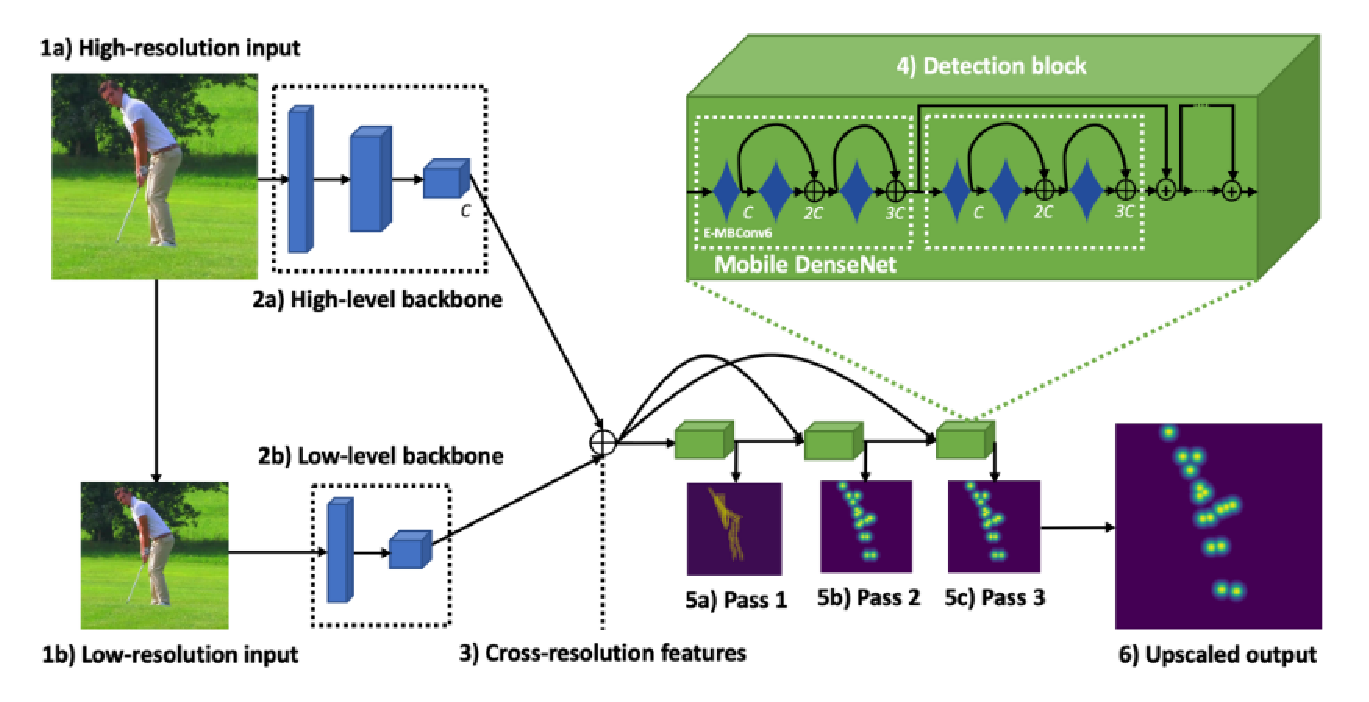
\includegraphics[scale=0.6]{EfficientPose}
	\caption{EfficientPose}
\end{center}
\end{figure}

The model takes in two inputs, one is the high-level features and second is the low-level features.
The low level features are obtained by downsampling an image to half of it's height and width using an average pooling layer.
The feature extractors here are initial layers of EfficientNet. For high level extractor, $\phi \in [0,7]$ and 
for the low level extractor $\phi \in [0,3]$.
\par
These extracted features and then concatendated together to obtain cross-resolution features.
This helps us to emphasize the important local factors in the image of interest.
\par
The input to the next phase of the model is the cross-resolution features obtained in the previous step.
Here the required keypoints are localized through an iterative process, where each
detection pass performs supervised prediction of output maps.
Each detection pass comprises a detection block
and a single 1 × 1 convolution for output prediction.
The detection blocks across all detection passes exhibit the
same basic architecture, comprising Mobile DenseNets.
Data from here is forwarded to the successive layers through skip connections.
Here, we also avoid downsampling of the output to preserve the resolution.
The original mobile convnets are modified by adding an E-swish activation function with $\beta$ value 1.25.
\par
The overall detection is performed in two rounds. Initially, the overall pose of the person is anticipated through a single pass of skeleton estimation. This helps especially when
there are multiple people present in the frame.
After the skeleton estimation is done two detection passes are performed to estimate heatmaps for points of interest.

\par
Another improvement on top of OpenPose is that, EfficientPose projects lower-resoltion image onto a higher resolution space using transposed convolution to allow an increased level of detail, whereas in OpenPose the heatmaps are
constrained to the lower space.
\section{Modules}
\subsection{EfficientNet}
EfficientNet \cite{Groos} is a CNN architecture that scales all dimensions, i.e, depth, width and resolution using a compound coefficient. The conventional practice is to scale these factors arbitrarily. Unlike this practice, EfficientNet method uniformly scales network dimensions using fixed scaling coefficients.  The justification for this approach is that as the input image gets bigger, then the network needs more layers to increase the receptive field and more channels to capture more fine patterns on the bigger image. Unlike regular ConvNet designs that focus on finding the best layer architecture, EfficientNet tried to expand the network length, width or resolution without changing the architecture predefined in the baseline network. 

The base network is based on inverted bottleneck blocks of MobileNetV2. EfficientNets also achieve state-of-the-art accuracy on multiple datasets, with comparatively fewer parameters.

\subsection{E-Swish}

Activation functions have a significant impact on training and testing the model against a problem. Rectified Linear Unit or ReLU is the most used activation function currently.  This project makes use of E- swish activation function, which is closely related with the Swish activation function, swish = x*sigmoid(x). E- swish is in a way used to generalize the swish function. 

E-swish = $\beta$ x * sigmoid(x). 

When $\beta$ = 1, it reverts to Swish. Like both Relu and swish, E-swish is unbounded above and bounded below. It is also smooth and non-monotonic. It can be implemented as a custom activation in popular deep learning libraries such as Keras and Tensorflow.

E- swish activation function has outperformed many well-known activation functions including ReLU and Swish. It has provided a 4.6\% accuracy improvement on cifar10 when compared to Relu and 0.6\% when compared to Swish.

\section{Accuracy Measures}
PCK is used as an accuracy metric that measures if the predicted keypoint and the true joint are within a certain distance threshold. The PCK is usually set with respect to the scale of the subject, which is enclosed within the bounding box.

The threshold can either be:
\begin{itemize}
    \item PCKh@0.5 is when the threshold = 50\% of the head bone link
    \item PCK@0.2 = Distance between predicted and true joint < 0.2 * torso diameter
    \item It alleviates the shorter limb problem since shorter limbs have smaller torsos and head bone links
\end{itemize}
\chapter{Datasets}
\section{MPII Human Pose Dataset}
MPII Human Pose dataset is a state of the art benchmark for evaluation of articulated human pose estimation. The dataset includes around 25K images containing over 40K people with annotated body joints. The images were systematically collected using an established taxonomy of every day human activities. Overall the dataset covers 410 human activities and each image is provided with an activity label. Each image was extracted from a YouTube video and provided with preceding and following un-annotated frames. In addition, for the test set we obtained richer annotations including body part occlusions and 3D torso and head orientations.
The model was trained primarily on this dataset.

\section{Leeds Sports Dataset}
This dataset contains 2000 pose annotated images of mostly sports people gathered from Flickr using the tags shown above. The images have been scaled such that the most prominent person is roughly 150 pixels in length. Each image has been annotated with 14 joint locations. Left and right joints are consistently labelled from a person-centric viewpoint. Attributions and Flickr URLs for the original images can be found in the JPEG comment field of each image file. 
The ordering of the joints are as follows:
\begin{enumerate}
	\item Right Ankle
	\item Right Knew
	\item Right Hip
	\item Left Hip
	\item Left Knee
	\item Left Ankle
	\item Right Wrist
	\item Right Elbow
	\item Right Shoulder
	\item Left Shoulder
	\item Left Elbow
	\item Left Wrist
	\item Neck
	\item Head Top
\end{enumerate}
\chapter{Results}

\begin{figure}[h!]
	\begin{center}
	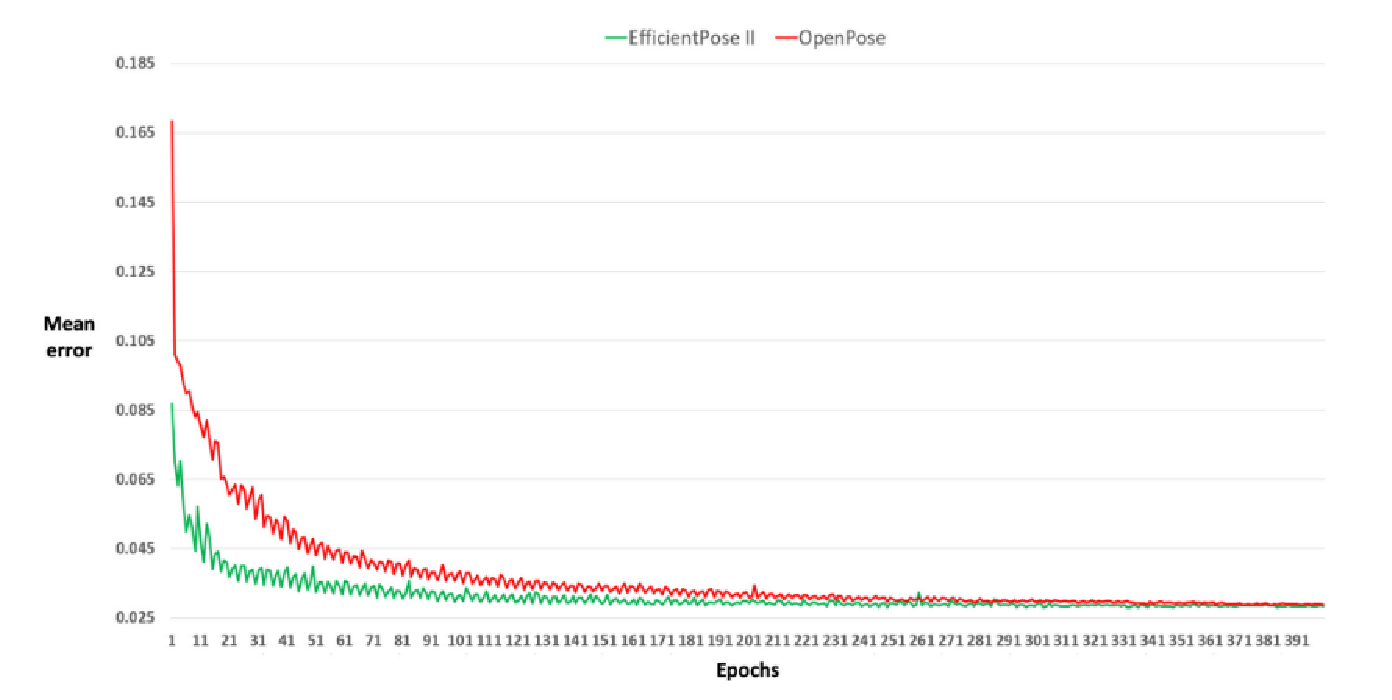
\includegraphics[scale=0.7]{TrainProgression}
	\caption{Convergence of mean error on OpenPose and EfficientPose}
\end{center}
\end{figure}
EfficientPose model has been compared with OpenPose on MPII dataset and Leeds sports dataset. All models of EfficientPose were optimized on LSP using SGD on mean squared error (MSE). 

The evaluation of model accuracy is measured using the PCKh metric, which is defined as the fraction of predictions residing within a distance from the ground truth location. The model has been evaluated on datasets, by using PCKh@50 as the standard performance metric. PCKh@10 has also been included to assess the model's ability to yield highly precise key point estimates.

It was observed that EfficientPose consistently outperformed OpenPose on efficiency, with considerable reduction in FLOPs and fewer number of parameters. Also, all model variants of EfficientPose achieved better high precision localization compared to OpenPose. It also showed rapid convergence during training phase, by converging earlier than OpenPose which requires up to 400 epochs before achieving proper convergence.

\chapter{Outputs}

\begin{figure}[h!]
	\begin{center}
	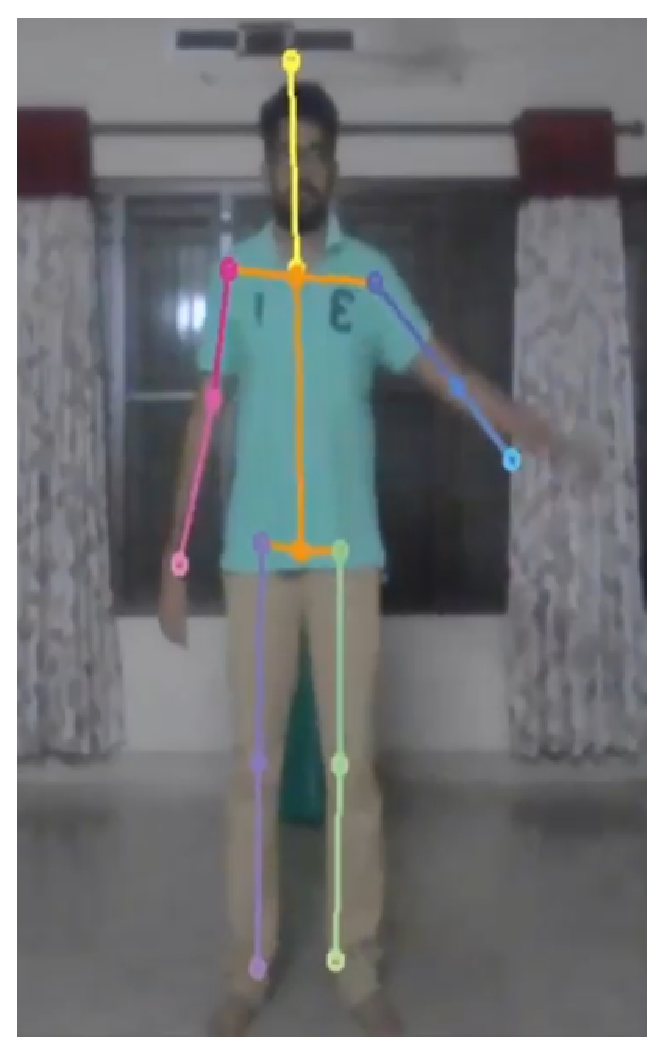
\includegraphics[scale=0.7]{op-1}
	\caption{Output 1}
\end{center}
\end{figure}

\begin{figure}[h!]
	\begin{center}
	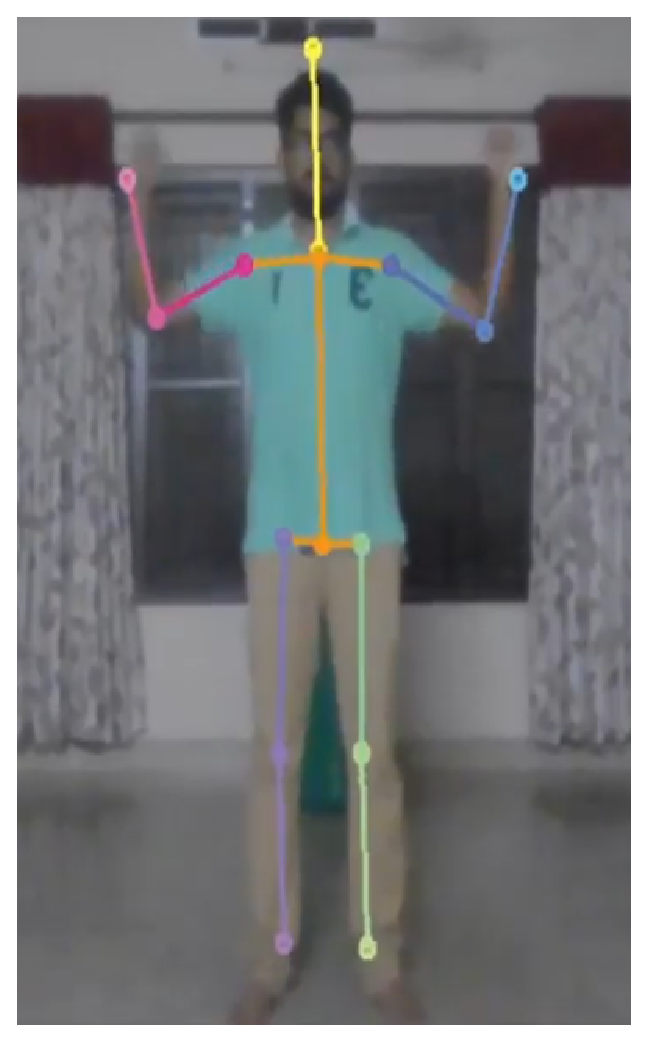
\includegraphics[scale=0.7]{pose-2}
	\caption{Output 2}
\end{center}
\end{figure}

\begin{figure}[h!]
	\begin{center}
	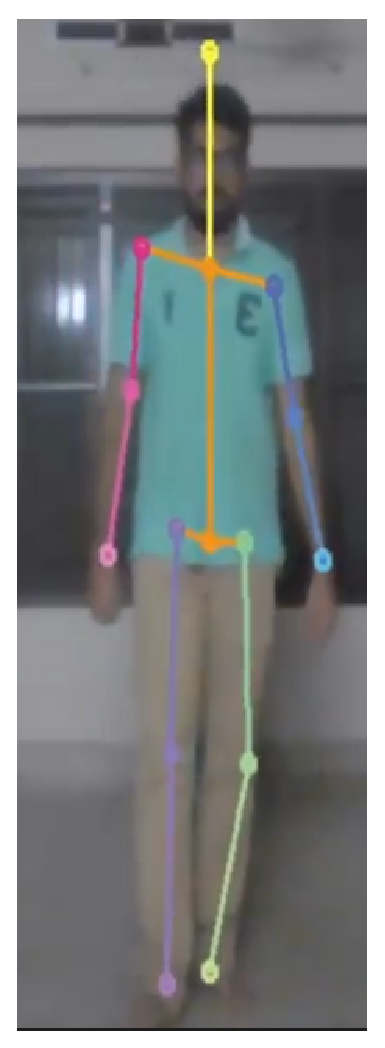
\includegraphics[scale=0.7]{pose-3}
	\caption{Output 3}
\end{center}
\end{figure}

\chapter{Conclusion}

By successfully exploiting the recent advances in convolutional neural networks, we have successfully made Single Person Pose-Estimation both more efficient and more accurate.
Due to this, many avenues of products in different fields may be developed that require real time pose estimation and hopefully it can be
used for wide ranging applications and products. The main advantage is the ability to run on edge devices which has been an achilles heel of
HPE for a long time.

\begin{thebibliography}{1}
\bibitem{Groos} EfficientPose: Scalable single-person pose estimation, ``Daniel Groos, Heri Ramampiaro, Espen AF Ihlen'' \url{https://link.springer.com/content/pdf/10.1007/s10489-020-01918-7.pdf}
\bibitem{knuth} EfficientNet: Rethinking Model Scaling for Convolutional Neural Networks, ``Mingxing Tan, Quoc V. Le'' \url{https://arxiv.org/pdf/1905.11946.pdf}.
\bibitem{Alcaide} E-swish: Adjusting Activations to Different Network Depths ``Eric Alcaide'' \url{https://arxiv.org/pdf/1801.07145.pdf}
\bibitem{d2l} Dive Into Deep Learning, \url{d2l.ai}
\end{thebibliography}

\begin{appendices}
\section{Source Code of EfficientPoseRT}
	\begin{lstlisting}
class KitModel(nn.Module):

    
    def __init__(self, weight_file):
        ....

    def forward(self, x):
        self.pass1_block1_mbconv1_skeleton_conv1_eswish_mul_x = torch.autograd.Variable(torch.Tensor([1.25]), requires_grad=False)
        self.pass1_block1_mbconv1_skeleton_dconv1_eswish_mul_x = torch.autograd.Variable(torch.Tensor([1.25]), requires_grad=False)
        self.pass1_block1_mbconv1_skeleton_se_se_squeeze_eswish_mul_x = torch.autograd.Variable(torch.Tensor([1.25]), requires_grad=False)
        self.pass1_block1_mbconv2_skeleton_conv1_eswish_mul_x = torch.autograd.Variable(torch.Tensor([1.25]), requires_grad=False)
        self.pass1_block1_mbconv2_skeleton_dconv1_eswish_mul_x = torch.autograd.Variable(torch.Tensor([1.25]), requires_grad=False)
        self.pass1_block1_mbconv2_skeleton_se_se_squeeze_eswish_mul_x = torch.autograd.Variable(torch.Tensor([1.25]), requires_grad=False)
        self.pass1_block1_mbconv3_skeleton_conv1_eswish_mul_x = torch.autograd.Variable(torch.Tensor([1.25]), requires_grad=False)
        self.pass1_block1_mbconv3_skeleton_dconv1_eswish_mul_x = torch.autograd.Variable(torch.Tensor([1.25]), requires_grad=False)
        self.pass1_block1_mbconv3_skeleton_se_se_squeeze_eswish_mul_x = torch.autograd.Variable(torch.Tensor([1.25]), requires_grad=False)
        self.pass2_block1_mbconv1_detection1_conv1_eswish_mul_x = torch.autograd.Variable(torch.Tensor([1.25]), requires_grad=False)
        self.pass2_block1_mbconv1_detection1_dconv1_eswish_mul_x = torch.autograd.Variable(torch.Tensor([1.25]), requires_grad=False)
        self.pass2_block1_mbconv1_detection1_se_se_squeeze_eswish_mul_x = torch.autograd.Variable(torch.Tensor([1.25]), requires_grad=False)
        self.pass2_block1_mbconv2_detection1_conv1_eswish_mul_x = torch.autograd.Variable(torch.Tensor([1.25]), requires_grad=False)
        self.pass2_block1_mbconv2_detection1_dconv1_eswish_mul_x = torch.autograd.Variable(torch.Tensor([1.25]), requires_grad=False)
        self.pass2_block1_mbconv2_detection1_se_se_squeeze_eswish_mul_x = torch.autograd.Variable(torch.Tensor([1.25]), requires_grad=False)
        self.pass2_block1_mbconv3_detection1_conv1_eswish_mul_x = torch.autograd.Variable(torch.Tensor([1.25]), requires_grad=False)
        self.pass2_block1_mbconv3_detection1_dconv1_eswish_mul_x = torch.autograd.Variable(torch.Tensor([1.25]), requires_grad=False)
        self.pass2_block1_mbconv3_detection1_se_se_squeeze_eswish_mul_x = torch.autograd.Variable(torch.Tensor([1.25]), requires_grad=False)
        self.pass3_block1_mbconv1_detection2_conv1_eswish_mul_x = torch.autograd.Variable(torch.Tensor([1.25]), requires_grad=False)
        self.pass3_block1_mbconv1_detection2_dconv1_eswish_mul_x = torch.autograd.Variable(torch.Tensor([1.25]), requires_grad=False)
        self.pass3_block1_mbconv1_detection2_se_se_squeeze_eswish_mul_x = torch.autograd.Variable(torch.Tensor([1.25]), requires_grad=False)
        self.pass3_block1_mbconv2_detection2_conv1_eswish_mul_x = torch.autograd.Variable(torch.Tensor([1.25]), requires_grad=False)
        self.pass3_block1_mbconv2_detection2_dconv1_eswish_mul_x = torch.autograd.Variable(torch.Tensor([1.25]), requires_grad=False)
        self.pass3_block1_mbconv2_detection2_se_se_squeeze_eswish_mul_x = torch.autograd.Variable(torch.Tensor([1.25]), requires_grad=False)
        self.pass3_block1_mbconv3_detection2_conv1_eswish_mul_x = torch.autograd.Variable(torch.Tensor([1.25]), requires_grad=False)
        self.pass3_block1_mbconv3_detection2_dconv1_eswish_mul_x = torch.autograd.Variable(torch.Tensor([1.25]), requires_grad=False)
        self.pass3_block1_mbconv3_detection2_se_se_squeeze_eswish_mul_x = torch.autograd.Variable(torch.Tensor([1.25]), requires_grad=False)
        stem_conv_res1_convolution_pad = F.pad(x, (0, 1, 0, 1))
        stem_conv_res1_convolution = self.stem_conv_res1_convolution(stem_conv_res1_convolution_pad)
        stem_bn_res1_FusedBatchNorm_1 = self.stem_bn_res1_FusedBatchNorm_1(stem_conv_res1_convolution)
        stem_activation_res1_Sigmoid = F.sigmoid(stem_bn_res1_FusedBatchNorm_1)
        stem_activation_res1_mul = stem_bn_res1_FusedBatchNorm_1 * stem_activation_res1_Sigmoid
        block1a_dwconv_res1_depthwise_pad = F.pad(stem_activation_res1_mul, (1, 1, 1, 1))
        block1a_dwconv_res1_depthwise = self.block1a_dwconv_res1_depthwise(block1a_dwconv_res1_depthwise_pad)
        block1a_bn_res1_FusedBatchNorm_1 = self.block1a_bn_res1_FusedBatchNorm_1(block1a_dwconv_res1_depthwise)
        block1a_activation_res1_Sigmoid = F.sigmoid(block1a_bn_res1_FusedBatchNorm_1)
        block1a_activation_res1_mul = block1a_bn_res1_FusedBatchNorm_1 * block1a_activation_res1_Sigmoid
        block1a_se_squeeze_res1_Mean = torch.mean(block1a_activation_res1_mul, 3, False)
        block1a_se_squeeze_res1_Mean = torch.mean(block1a_se_squeeze_res1_Mean, 2, False)
        block1a_se_reshape_res1_Shape = torch.Tensor(list(block1a_se_squeeze_res1_Mean.size()))
        block1a_se_reshape_res1_Reshape = torch.reshape(input = block1a_se_squeeze_res1_Mean, shape = (-1,32,1,1))#(-1,1,1,32))
        block1a_se_reshape_res1_strided_slice = block1a_se_reshape_res1_Shape[0:1]
        block1a_se_reduce_res1_convolution = self.block1a_se_reduce_res1_convolution(block1a_se_reshape_res1_Reshape)
        block1a_se_reduce_swish_res1_Sigmoid = F.sigmoid(block1a_se_reduce_res1_convolution)
        block1a_se_reduce_swish_res1_mul = block1a_se_reduce_res1_convolution * block1a_se_reduce_swish_res1_Sigmoid
        block1a_se_expand_res1_convolution = self.block1a_se_expand_res1_convolution(block1a_se_reduce_swish_res1_mul)
        block1a_se_expand_res1_Sigmoid = F.sigmoid(block1a_se_expand_res1_convolution)
        block1a_se_excite_res1_mul = block1a_activation_res1_mul * block1a_se_expand_res1_Sigmoid
        block1a_project_conv_res1_convolution = self.block1a_project_conv_res1_convolution(block1a_se_excite_res1_mul)
        block1a_project_bn_res1_FusedBatchNorm_1 = self.block1a_project_bn_res1_FusedBatchNorm_1(block1a_project_conv_res1_convolution)
        block2a_expand_conv_res1_convolution = self.block2a_expand_conv_res1_convolution(block1a_project_bn_res1_FusedBatchNorm_1)
        block2a_expand_bn_res1_FusedBatchNorm_1 = self.block2a_expand_bn_res1_FusedBatchNorm_1(block2a_expand_conv_res1_convolution)
        block2a_expand_activation_res1_Sigmoid = F.sigmoid(block2a_expand_bn_res1_FusedBatchNorm_1)
        block2a_expand_activation_res1_mul = block2a_expand_bn_res1_FusedBatchNorm_1 * block2a_expand_activation_res1_Sigmoid
        block2a_dwconv_res1_depthwise_pad = F.pad(block2a_expand_activation_res1_mul, (0, 1, 0, 1))
        block2a_dwconv_res1_depthwise = self.block2a_dwconv_res1_depthwise(block2a_dwconv_res1_depthwise_pad)
        block2a_bn_res1_FusedBatchNorm_1 = self.block2a_bn_res1_FusedBatchNorm_1(block2a_dwconv_res1_depthwise)
        block2a_activation_res1_Sigmoid = F.sigmoid(block2a_bn_res1_FusedBatchNorm_1)
        block2a_activation_res1_mul = block2a_bn_res1_FusedBatchNorm_1 * block2a_activation_res1_Sigmoid
        block2a_se_squeeze_res1_Mean = torch.mean(block2a_activation_res1_mul, 3, False)
        block2a_se_squeeze_res1_Mean = torch.mean(block2a_se_squeeze_res1_Mean, 2, False)
        block2a_se_reshape_res1_Shape = torch.Tensor(list(block2a_se_squeeze_res1_Mean.size()))
        block2a_se_reshape_res1_Reshape = torch.reshape(input = block2a_se_squeeze_res1_Mean, shape = (-1,96,1,1))#(-1,1,1,96))
        block2a_se_reshape_res1_strided_slice = block2a_se_reshape_res1_Shape[0:1]
        block2a_se_reduce_res1_convolution = self.block2a_se_reduce_res1_convolution(block2a_se_reshape_res1_Reshape)
        block2a_se_reduce_swish_res1_Sigmoid = F.sigmoid(block2a_se_reduce_res1_convolution)
        block2a_se_reduce_swish_res1_mul = block2a_se_reduce_res1_convolution * block2a_se_reduce_swish_res1_Sigmoid
        block2a_se_expand_res1_convolution = self.block2a_se_expand_res1_convolution(block2a_se_reduce_swish_res1_mul)
        block2a_se_expand_res1_Sigmoid = F.sigmoid(block2a_se_expand_res1_convolution)
        block2a_se_excite_res1_mul = block2a_activation_res1_mul * block2a_se_expand_res1_Sigmoid
        block2a_project_conv_res1_convolution = self.block2a_project_conv_res1_convolution(block2a_se_excite_res1_mul)
        block2a_project_bn_res1_FusedBatchNorm_1 = self.block2a_project_bn_res1_FusedBatchNorm_1(block2a_project_conv_res1_convolution)
        block2b_expand_conv_res1_convolution = self.block2b_expand_conv_res1_convolution(block2a_project_bn_res1_FusedBatchNorm_1)
        block2b_expand_bn_res1_FusedBatchNorm_1 = self.block2b_expand_bn_res1_FusedBatchNorm_1(block2b_expand_conv_res1_convolution)
        block2b_expand_activation_res1_Sigmoid = F.sigmoid(block2b_expand_bn_res1_FusedBatchNorm_1)
        block2b_expand_activation_res1_mul = block2b_expand_bn_res1_FusedBatchNorm_1 * block2b_expand_activation_res1_Sigmoid
        block2b_dwconv_res1_depthwise_pad = F.pad(block2b_expand_activation_res1_mul, (1, 1, 1, 1))
        block2b_dwconv_res1_depthwise = self.block2b_dwconv_res1_depthwise(block2b_dwconv_res1_depthwise_pad)
        block2b_bn_res1_FusedBatchNorm_1 = self.block2b_bn_res1_FusedBatchNorm_1(block2b_dwconv_res1_depthwise)
        block2b_activation_res1_Sigmoid = F.sigmoid(block2b_bn_res1_FusedBatchNorm_1)
        block2b_activation_res1_mul = block2b_bn_res1_FusedBatchNorm_1 * block2b_activation_res1_Sigmoid
        block2b_se_squeeze_res1_Mean = torch.mean(block2b_activation_res1_mul, 3, False)
        block2b_se_squeeze_res1_Mean = torch.mean(block2b_se_squeeze_res1_Mean, 2, False)
        block2b_se_reshape_res1_Shape = torch.Tensor(list(block2b_se_squeeze_res1_Mean.size()))
        block2b_se_reshape_res1_Reshape = torch.reshape(input = block2b_se_squeeze_res1_Mean, shape = (-1,144,1,1))#(-1,1,1,144))
        block2b_se_reshape_res1_strided_slice = block2b_se_reshape_res1_Shape[0:1]
        block2b_se_reduce_res1_convolution = self.block2b_se_reduce_res1_convolution(block2b_se_reshape_res1_Reshape)
        block2b_se_reduce_swish_res1_Sigmoid = F.sigmoid(block2b_se_reduce_res1_convolution)
        block2b_se_reduce_swish_res1_mul = block2b_se_reduce_res1_convolution * block2b_se_reduce_swish_res1_Sigmoid
        block2b_se_expand_res1_convolution = self.block2b_se_expand_res1_convolution(block2b_se_reduce_swish_res1_mul)
        block2b_se_expand_res1_Sigmoid = F.sigmoid(block2b_se_expand_res1_convolution)
        block2b_se_excite_res1_mul = block2b_activation_res1_mul * block2b_se_expand_res1_Sigmoid
        block2b_project_conv_res1_convolution = self.block2b_project_conv_res1_convolution(block2b_se_excite_res1_mul)
        block2b_project_bn_res1_FusedBatchNorm_1 = self.block2b_project_bn_res1_FusedBatchNorm_1(block2b_project_conv_res1_convolution)
        block2b_add_res1_add = block2b_project_bn_res1_FusedBatchNorm_1 + block2a_project_bn_res1_FusedBatchNorm_1
        block3a_expand_conv_res1_convolution = self.block3a_expand_conv_res1_convolution(block2b_add_res1_add)
        block3a_expand_bn_res1_FusedBatchNorm_1 = self.block3a_expand_bn_res1_FusedBatchNorm_1(block3a_expand_conv_res1_convolution)
        block3a_expand_activation_res1_Sigmoid = F.sigmoid(block3a_expand_bn_res1_FusedBatchNorm_1)
        block3a_expand_activation_res1_mul = block3a_expand_bn_res1_FusedBatchNorm_1 * block3a_expand_activation_res1_Sigmoid
        block3a_dwconv_res1_depthwise_pad = F.pad(block3a_expand_activation_res1_mul, (1, 2, 1, 2))
        block3a_dwconv_res1_depthwise = self.block3a_dwconv_res1_depthwise(block3a_dwconv_res1_depthwise_pad)
        block3a_bn_res1_FusedBatchNorm_1 = self.block3a_bn_res1_FusedBatchNorm_1(block3a_dwconv_res1_depthwise)
        block3a_activation_res1_Sigmoid = F.sigmoid(block3a_bn_res1_FusedBatchNorm_1)
        block3a_activation_res1_mul = block3a_bn_res1_FusedBatchNorm_1 * block3a_activation_res1_Sigmoid
        block3a_se_squeeze_res1_Mean = torch.mean(block3a_activation_res1_mul, 3, False)
        block3a_se_squeeze_res1_Mean = torch.mean(block3a_se_squeeze_res1_Mean, 2, False)
        block3a_se_reshape_res1_Shape = torch.Tensor(list(block3a_se_squeeze_res1_Mean.size()))
        block3a_se_reshape_res1_Reshape = torch.reshape(input = block3a_se_squeeze_res1_Mean, shape = (-1,144,1,1))#(-1,1,1,144))
        block3a_se_reshape_res1_strided_slice = block3a_se_reshape_res1_Shape[0:1]
        block3a_se_reduce_res1_convolution = self.block3a_se_reduce_res1_convolution(block3a_se_reshape_res1_Reshape)
        block3a_se_reduce_swish_res1_Sigmoid = F.sigmoid(block3a_se_reduce_res1_convolution)
        block3a_se_reduce_swish_res1_mul = block3a_se_reduce_res1_convolution * block3a_se_reduce_swish_res1_Sigmoid
        block3a_se_expand_res1_convolution = self.block3a_se_expand_res1_convolution(block3a_se_reduce_swish_res1_mul)
        block3a_se_expand_res1_Sigmoid = F.sigmoid(block3a_se_expand_res1_convolution)
        block3a_se_excite_res1_mul = block3a_activation_res1_mul * block3a_se_expand_res1_Sigmoid
        block3a_project_conv_res1_convolution = self.block3a_project_conv_res1_convolution(block3a_se_excite_res1_mul)
        block3a_project_bn_res1_FusedBatchNorm_1 = self.block3a_project_bn_res1_FusedBatchNorm_1(block3a_project_conv_res1_convolution)
        block3b_expand_conv_res1_convolution = self.block3b_expand_conv_res1_convolution(block3a_project_bn_res1_FusedBatchNorm_1)
        block3b_expand_bn_res1_FusedBatchNorm_1 = self.block3b_expand_bn_res1_FusedBatchNorm_1(block3b_expand_conv_res1_convolution)
        block3b_expand_activation_res1_Sigmoid = F.sigmoid(block3b_expand_bn_res1_FusedBatchNorm_1)
        block3b_expand_activation_res1_mul = block3b_expand_bn_res1_FusedBatchNorm_1 * block3b_expand_activation_res1_Sigmoid
        block3b_dwconv_res1_depthwise_pad = F.pad(block3b_expand_activation_res1_mul, (2, 2, 2, 2))
        block3b_dwconv_res1_depthwise = self.block3b_dwconv_res1_depthwise(block3b_dwconv_res1_depthwise_pad)
        block3b_bn_res1_FusedBatchNorm_1 = self.block3b_bn_res1_FusedBatchNorm_1(block3b_dwconv_res1_depthwise)
        block3b_activation_res1_Sigmoid = F.sigmoid(block3b_bn_res1_FusedBatchNorm_1)
        block3b_activation_res1_mul = block3b_bn_res1_FusedBatchNorm_1 * block3b_activation_res1_Sigmoid
        block3b_se_squeeze_res1_Mean = torch.mean(block3b_activation_res1_mul, 3, False)
        block3b_se_squeeze_res1_Mean = torch.mean(block3b_se_squeeze_res1_Mean, 2, False)
        block3b_se_reshape_res1_Shape = torch.Tensor(list(block3b_se_squeeze_res1_Mean.size()))
        block3b_se_reshape_res1_Reshape = torch.reshape(input = block3b_se_squeeze_res1_Mean, shape = (-1,240,1,1))#(-1,1,1,240))
        block3b_se_reshape_res1_strided_slice = block3b_se_reshape_res1_Shape[0:1]
        block3b_se_reduce_res1_convolution = self.block3b_se_reduce_res1_convolution(block3b_se_reshape_res1_Reshape)
        block3b_se_reduce_swish_res1_Sigmoid = F.sigmoid(block3b_se_reduce_res1_convolution)
        block3b_se_reduce_swish_res1_mul = block3b_se_reduce_res1_convolution * block3b_se_reduce_swish_res1_Sigmoid
        block3b_se_expand_res1_convolution = self.block3b_se_expand_res1_convolution(block3b_se_reduce_swish_res1_mul)
        block3b_se_expand_res1_Sigmoid = F.sigmoid(block3b_se_expand_res1_convolution)
        block3b_se_excite_res1_mul = block3b_activation_res1_mul * block3b_se_expand_res1_Sigmoid
        block3b_project_conv_res1_convolution = self.block3b_project_conv_res1_convolution(block3b_se_excite_res1_mul)
        block3b_project_bn_res1_FusedBatchNorm_1 = self.block3b_project_bn_res1_FusedBatchNorm_1(block3b_project_conv_res1_convolution)
        block3b_add_res1_add = block3b_project_bn_res1_FusedBatchNorm_1 + block3a_project_bn_res1_FusedBatchNorm_1
        pass1_block1_mbconv1_skeleton_conv1_convolution = self.pass1_block1_mbconv1_skeleton_conv1_convolution(block3b_add_res1_add)
        pass1_block1_mbconv1_skeleton_conv1_bn_FusedBatchNorm_1 = self.pass1_block1_mbconv1_skeleton_conv1_bn_FusedBatchNorm_1(pass1_block1_mbconv1_skeleton_conv1_convolution)
        pass1_block1_mbconv1_skeleton_conv1_eswish_mul = self.pass1_block1_mbconv1_skeleton_conv1_eswish_mul_x * pass1_block1_mbconv1_skeleton_conv1_bn_FusedBatchNorm_1
        pass1_block1_mbconv1_skeleton_conv1_eswish_Sigmoid = F.sigmoid(pass1_block1_mbconv1_skeleton_conv1_bn_FusedBatchNorm_1)
        pass1_block1_mbconv1_skeleton_conv1_eswish_mul_1 = pass1_block1_mbconv1_skeleton_conv1_eswish_mul * pass1_block1_mbconv1_skeleton_conv1_eswish_Sigmoid
        pass1_block1_mbconv1_skeleton_dconv1_depthwise_pad = F.pad(pass1_block1_mbconv1_skeleton_conv1_eswish_mul_1, (2, 2, 2, 2))
        pass1_block1_mbconv1_skeleton_dconv1_depthwise = self.pass1_block1_mbconv1_skeleton_dconv1_depthwise(pass1_block1_mbconv1_skeleton_dconv1_depthwise_pad)
        pass1_block1_mbconv1_skeleton_dconv1_bn_FusedBatchNorm_1 = self.pass1_block1_mbconv1_skeleton_dconv1_bn_FusedBatchNorm_1(pass1_block1_mbconv1_skeleton_dconv1_depthwise)
        pass1_block1_mbconv1_skeleton_dconv1_eswish_mul = self.pass1_block1_mbconv1_skeleton_dconv1_eswish_mul_x * pass1_block1_mbconv1_skeleton_dconv1_bn_FusedBatchNorm_1
        pass1_block1_mbconv1_skeleton_dconv1_eswish_Sigmoid = F.sigmoid(pass1_block1_mbconv1_skeleton_dconv1_bn_FusedBatchNorm_1)
        pass1_block1_mbconv1_skeleton_dconv1_eswish_mul_1 = pass1_block1_mbconv1_skeleton_dconv1_eswish_mul * pass1_block1_mbconv1_skeleton_dconv1_eswish_Sigmoid
        pass1_block1_mbconv1_skeleton_se_se_squeeze_lambda_Mean = torch.mean(pass1_block1_mbconv1_skeleton_dconv1_eswish_mul_1, 3, True)
        pass1_block1_mbconv1_skeleton_se_se_squeeze_lambda_Mean = torch.mean(pass1_block1_mbconv1_skeleton_se_se_squeeze_lambda_Mean, 2, True)
        pass1_block1_mbconv1_skeleton_se_se_squeeze_conv_convolution = self.pass1_block1_mbconv1_skeleton_se_se_squeeze_conv_convolution(pass1_block1_mbconv1_skeleton_se_se_squeeze_lambda_Mean)
        pass1_block1_mbconv1_skeleton_se_se_squeeze_eswish_mul = self.pass1_block1_mbconv1_skeleton_se_se_squeeze_eswish_mul_x * pass1_block1_mbconv1_skeleton_se_se_squeeze_conv_convolution
        pass1_block1_mbconv1_skeleton_se_se_squeeze_eswish_Sigmoid = F.sigmoid(pass1_block1_mbconv1_skeleton_se_se_squeeze_conv_convolution)
        pass1_block1_mbconv1_skeleton_se_se_squeeze_eswish_mul_1 = pass1_block1_mbconv1_skeleton_se_se_squeeze_eswish_mul * pass1_block1_mbconv1_skeleton_se_se_squeeze_eswish_Sigmoid
        pass1_block1_mbconv1_skeleton_se_se_excite_conv_convolution = self.pass1_block1_mbconv1_skeleton_se_se_excite_conv_convolution(pass1_block1_mbconv1_skeleton_se_se_squeeze_eswish_mul_1)
        pass1_block1_mbconv1_skeleton_se_se_excite_sigmoid_Sigmoid = F.sigmoid(pass1_block1_mbconv1_skeleton_se_se_excite_conv_convolution)
        pass1_block1_mbconv1_skeleton_se_se_multiply_mul = pass1_block1_mbconv1_skeleton_se_se_excite_sigmoid_Sigmoid * pass1_block1_mbconv1_skeleton_dconv1_eswish_mul_1
        pass1_block1_mbconv1_skeleton_conv2_convolution = self.pass1_block1_mbconv1_skeleton_conv2_convolution(pass1_block1_mbconv1_skeleton_se_se_multiply_mul)
        pass1_block1_mbconv1_skeleton_conv2_bn_FusedBatchNorm_1 = self.pass1_block1_mbconv1_skeleton_conv2_bn_FusedBatchNorm_1(pass1_block1_mbconv1_skeleton_conv2_convolution)
        pass1_block1_mbconv2_skeleton_conv1_convolution = self.pass1_block1_mbconv2_skeleton_conv1_convolution(pass1_block1_mbconv1_skeleton_conv2_bn_FusedBatchNorm_1)
        pass1_block1_mbconv2_skeleton_conv1_bn_FusedBatchNorm_1 = self.pass1_block1_mbconv2_skeleton_conv1_bn_FusedBatchNorm_1(pass1_block1_mbconv2_skeleton_conv1_convolution)
        pass1_block1_mbconv2_skeleton_conv1_eswish_mul = self.pass1_block1_mbconv2_skeleton_conv1_eswish_mul_x * pass1_block1_mbconv2_skeleton_conv1_bn_FusedBatchNorm_1
        pass1_block1_mbconv2_skeleton_conv1_eswish_Sigmoid = F.sigmoid(pass1_block1_mbconv2_skeleton_conv1_bn_FusedBatchNorm_1)
        pass1_block1_mbconv2_skeleton_conv1_eswish_mul_1 = pass1_block1_mbconv2_skeleton_conv1_eswish_mul * pass1_block1_mbconv2_skeleton_conv1_eswish_Sigmoid
        pass1_block1_mbconv2_skeleton_dconv1_depthwise_pad = F.pad(pass1_block1_mbconv2_skeleton_conv1_eswish_mul_1, (2, 2, 2, 2))
        pass1_block1_mbconv2_skeleton_dconv1_depthwise = self.pass1_block1_mbconv2_skeleton_dconv1_depthwise(pass1_block1_mbconv2_skeleton_dconv1_depthwise_pad)
        pass1_block1_mbconv2_skeleton_dconv1_bn_FusedBatchNorm_1 = self.pass1_block1_mbconv2_skeleton_dconv1_bn_FusedBatchNorm_1(pass1_block1_mbconv2_skeleton_dconv1_depthwise)
        pass1_block1_mbconv2_skeleton_dconv1_eswish_mul = self.pass1_block1_mbconv2_skeleton_dconv1_eswish_mul_x * pass1_block1_mbconv2_skeleton_dconv1_bn_FusedBatchNorm_1
        pass1_block1_mbconv2_skeleton_dconv1_eswish_Sigmoid = F.sigmoid(pass1_block1_mbconv2_skeleton_dconv1_bn_FusedBatchNorm_1)
        pass1_block1_mbconv2_skeleton_dconv1_eswish_mul_1 = pass1_block1_mbconv2_skeleton_dconv1_eswish_mul * pass1_block1_mbconv2_skeleton_dconv1_eswish_Sigmoid
        pass1_block1_mbconv2_skeleton_se_se_squeeze_lambda_Mean = torch.mean(pass1_block1_mbconv2_skeleton_dconv1_eswish_mul_1, 3, True)
        pass1_block1_mbconv2_skeleton_se_se_squeeze_lambda_Mean = torch.mean(pass1_block1_mbconv2_skeleton_se_se_squeeze_lambda_Mean, 2, True)
        pass1_block1_mbconv2_skeleton_se_se_squeeze_conv_convolution = self.pass1_block1_mbconv2_skeleton_se_se_squeeze_conv_convolution(pass1_block1_mbconv2_skeleton_se_se_squeeze_lambda_Mean)
        pass1_block1_mbconv2_skeleton_se_se_squeeze_eswish_mul = self.pass1_block1_mbconv2_skeleton_se_se_squeeze_eswish_mul_x * pass1_block1_mbconv2_skeleton_se_se_squeeze_conv_convolution
        pass1_block1_mbconv2_skeleton_se_se_squeeze_eswish_Sigmoid = F.sigmoid(pass1_block1_mbconv2_skeleton_se_se_squeeze_conv_convolution)
        pass1_block1_mbconv2_skeleton_se_se_squeeze_eswish_mul_1 = pass1_block1_mbconv2_skeleton_se_se_squeeze_eswish_mul * pass1_block1_mbconv2_skeleton_se_se_squeeze_eswish_Sigmoid
        pass1_block1_mbconv2_skeleton_se_se_excite_conv_convolution = self.pass1_block1_mbconv2_skeleton_se_se_excite_conv_convolution(pass1_block1_mbconv2_skeleton_se_se_squeeze_eswish_mul_1)
        pass1_block1_mbconv2_skeleton_se_se_excite_sigmoid_Sigmoid = F.sigmoid(pass1_block1_mbconv2_skeleton_se_se_excite_conv_convolution)
        pass1_block1_mbconv2_skeleton_se_se_multiply_mul = pass1_block1_mbconv2_skeleton_se_se_excite_sigmoid_Sigmoid * pass1_block1_mbconv2_skeleton_dconv1_eswish_mul_1
        pass1_block1_mbconv2_skeleton_conv2_convolution = self.pass1_block1_mbconv2_skeleton_conv2_convolution(pass1_block1_mbconv2_skeleton_se_se_multiply_mul)
        pass1_block1_mbconv2_skeleton_conv2_bn_FusedBatchNorm_1 = self.pass1_block1_mbconv2_skeleton_conv2_bn_FusedBatchNorm_1(pass1_block1_mbconv2_skeleton_conv2_convolution)
        pass1_block1_mbconv2_skeleton_dense_concat = torch.cat((pass1_block1_mbconv2_skeleton_conv2_bn_FusedBatchNorm_1, pass1_block1_mbconv1_skeleton_conv2_bn_FusedBatchNorm_1), 1)
        pass1_block1_mbconv3_skeleton_conv1_convolution = self.pass1_block1_mbconv3_skeleton_conv1_convolution(pass1_block1_mbconv2_skeleton_dense_concat)
        pass1_block1_mbconv3_skeleton_conv1_bn_FusedBatchNorm_1 = self.pass1_block1_mbconv3_skeleton_conv1_bn_FusedBatchNorm_1(pass1_block1_mbconv3_skeleton_conv1_convolution)
        pass1_block1_mbconv3_skeleton_conv1_eswish_mul = self.pass1_block1_mbconv3_skeleton_conv1_eswish_mul_x * pass1_block1_mbconv3_skeleton_conv1_bn_FusedBatchNorm_1
        pass1_block1_mbconv3_skeleton_conv1_eswish_Sigmoid = F.sigmoid(pass1_block1_mbconv3_skeleton_conv1_bn_FusedBatchNorm_1)
        pass1_block1_mbconv3_skeleton_conv1_eswish_mul_1 = pass1_block1_mbconv3_skeleton_conv1_eswish_mul * pass1_block1_mbconv3_skeleton_conv1_eswish_Sigmoid
        pass1_block1_mbconv3_skeleton_dconv1_depthwise_pad = F.pad(pass1_block1_mbconv3_skeleton_conv1_eswish_mul_1, (2, 2, 2, 2))
        pass1_block1_mbconv3_skeleton_dconv1_depthwise = self.pass1_block1_mbconv3_skeleton_dconv1_depthwise(pass1_block1_mbconv3_skeleton_dconv1_depthwise_pad)
        pass1_block1_mbconv3_skeleton_dconv1_bn_FusedBatchNorm_1 = self.pass1_block1_mbconv3_skeleton_dconv1_bn_FusedBatchNorm_1(pass1_block1_mbconv3_skeleton_dconv1_depthwise)
        pass1_block1_mbconv3_skeleton_dconv1_eswish_mul = self.pass1_block1_mbconv3_skeleton_dconv1_eswish_mul_x * pass1_block1_mbconv3_skeleton_dconv1_bn_FusedBatchNorm_1
        pass1_block1_mbconv3_skeleton_dconv1_eswish_Sigmoid = F.sigmoid(pass1_block1_mbconv3_skeleton_dconv1_bn_FusedBatchNorm_1)
        pass1_block1_mbconv3_skeleton_dconv1_eswish_mul_1 = pass1_block1_mbconv3_skeleton_dconv1_eswish_mul * pass1_block1_mbconv3_skeleton_dconv1_eswish_Sigmoid
        pass1_block1_mbconv3_skeleton_se_se_squeeze_lambda_Mean = torch.mean(pass1_block1_mbconv3_skeleton_dconv1_eswish_mul_1, 3, True)
        pass1_block1_mbconv3_skeleton_se_se_squeeze_lambda_Mean = torch.mean(pass1_block1_mbconv3_skeleton_se_se_squeeze_lambda_Mean, 2, True)
        pass1_block1_mbconv3_skeleton_se_se_squeeze_conv_convolution = self.pass1_block1_mbconv3_skeleton_se_se_squeeze_conv_convolution(pass1_block1_mbconv3_skeleton_se_se_squeeze_lambda_Mean)
        pass1_block1_mbconv3_skeleton_se_se_squeeze_eswish_mul = self.pass1_block1_mbconv3_skeleton_se_se_squeeze_eswish_mul_x * pass1_block1_mbconv3_skeleton_se_se_squeeze_conv_convolution
        pass1_block1_mbconv3_skeleton_se_se_squeeze_eswish_Sigmoid = F.sigmoid(pass1_block1_mbconv3_skeleton_se_se_squeeze_conv_convolution)
        pass1_block1_mbconv3_skeleton_se_se_squeeze_eswish_mul_1 = pass1_block1_mbconv3_skeleton_se_se_squeeze_eswish_mul * pass1_block1_mbconv3_skeleton_se_se_squeeze_eswish_Sigmoid
        pass1_block1_mbconv3_skeleton_se_se_excite_conv_convolution = self.pass1_block1_mbconv3_skeleton_se_se_excite_conv_convolution(pass1_block1_mbconv3_skeleton_se_se_squeeze_eswish_mul_1)
        pass1_block1_mbconv3_skeleton_se_se_excite_sigmoid_Sigmoid = F.sigmoid(pass1_block1_mbconv3_skeleton_se_se_excite_conv_convolution)
        pass1_block1_mbconv3_skeleton_se_se_multiply_mul = pass1_block1_mbconv3_skeleton_se_se_excite_sigmoid_Sigmoid * pass1_block1_mbconv3_skeleton_dconv1_eswish_mul_1
        pass1_block1_mbconv3_skeleton_conv2_convolution = self.pass1_block1_mbconv3_skeleton_conv2_convolution(pass1_block1_mbconv3_skeleton_se_se_multiply_mul)
        pass1_block1_mbconv3_skeleton_conv2_bn_FusedBatchNorm_1 = self.pass1_block1_mbconv3_skeleton_conv2_bn_FusedBatchNorm_1(pass1_block1_mbconv3_skeleton_conv2_convolution)
        pass1_block1_mbconv3_skeleton_dense_concat = torch.cat((pass1_block1_mbconv3_skeleton_conv2_bn_FusedBatchNorm_1, pass1_block1_mbconv2_skeleton_dense_concat), 1)
        concatenate_1_concat = torch.cat((pass1_block1_mbconv3_skeleton_dense_concat, block3b_add_res1_add), 1)
        pass2_block1_mbconv1_detection1_conv1_convolution = self.pass2_block1_mbconv1_detection1_conv1_convolution(concatenate_1_concat)
        pass2_block1_mbconv1_detection1_conv1_bn_FusedBatchNorm_1 = self.pass2_block1_mbconv1_detection1_conv1_bn_FusedBatchNorm_1(pass2_block1_mbconv1_detection1_conv1_convolution)
        pass2_block1_mbconv1_detection1_conv1_eswish_mul = self.pass2_block1_mbconv1_detection1_conv1_eswish_mul_x * pass2_block1_mbconv1_detection1_conv1_bn_FusedBatchNorm_1
        pass2_block1_mbconv1_detection1_conv1_eswish_Sigmoid = F.sigmoid(pass2_block1_mbconv1_detection1_conv1_bn_FusedBatchNorm_1)
        pass2_block1_mbconv1_detection1_conv1_eswish_mul_1 = pass2_block1_mbconv1_detection1_conv1_eswish_mul * pass2_block1_mbconv1_detection1_conv1_eswish_Sigmoid
        pass2_block1_mbconv1_detection1_dconv1_depthwise_pad = F.pad(pass2_block1_mbconv1_detection1_conv1_eswish_mul_1, (2, 2, 2, 2))
        pass2_block1_mbconv1_detection1_dconv1_depthwise = self.pass2_block1_mbconv1_detection1_dconv1_depthwise(pass2_block1_mbconv1_detection1_dconv1_depthwise_pad)
        pass2_block1_mbconv1_detection1_dconv1_bn_FusedBatchNorm_1 = self.pass2_block1_mbconv1_detection1_dconv1_bn_FusedBatchNorm_1(pass2_block1_mbconv1_detection1_dconv1_depthwise)
        pass2_block1_mbconv1_detection1_dconv1_eswish_mul = self.pass2_block1_mbconv1_detection1_dconv1_eswish_mul_x * pass2_block1_mbconv1_detection1_dconv1_bn_FusedBatchNorm_1
        pass2_block1_mbconv1_detection1_dconv1_eswish_Sigmoid = F.sigmoid(pass2_block1_mbconv1_detection1_dconv1_bn_FusedBatchNorm_1)
        pass2_block1_mbconv1_detection1_dconv1_eswish_mul_1 = pass2_block1_mbconv1_detection1_dconv1_eswish_mul * pass2_block1_mbconv1_detection1_dconv1_eswish_Sigmoid
        pass2_block1_mbconv1_detection1_se_se_squeeze_lambda_Mean = torch.mean(pass2_block1_mbconv1_detection1_dconv1_eswish_mul_1, 3, True)
        pass2_block1_mbconv1_detection1_se_se_squeeze_lambda_Mean = torch.mean(pass2_block1_mbconv1_detection1_se_se_squeeze_lambda_Mean, 2, True)
        pass2_block1_mbconv1_detection1_se_se_squeeze_conv_convolution = self.pass2_block1_mbconv1_detection1_se_se_squeeze_conv_convolution(pass2_block1_mbconv1_detection1_se_se_squeeze_lambda_Mean)
        pass2_block1_mbconv1_detection1_se_se_squeeze_eswish_mul = self.pass2_block1_mbconv1_detection1_se_se_squeeze_eswish_mul_x * pass2_block1_mbconv1_detection1_se_se_squeeze_conv_convolution
        pass2_block1_mbconv1_detection1_se_se_squeeze_eswish_Sigmoid = F.sigmoid(pass2_block1_mbconv1_detection1_se_se_squeeze_conv_convolution)
        pass2_block1_mbconv1_detection1_se_se_squeeze_eswish_mul_1 = pass2_block1_mbconv1_detection1_se_se_squeeze_eswish_mul * pass2_block1_mbconv1_detection1_se_se_squeeze_eswish_Sigmoid
        pass2_block1_mbconv1_detection1_se_se_excite_conv_convolution = self.pass2_block1_mbconv1_detection1_se_se_excite_conv_convolution(pass2_block1_mbconv1_detection1_se_se_squeeze_eswish_mul_1)
        pass2_block1_mbconv1_detection1_se_se_excite_sigmoid_Sigmoid = F.sigmoid(pass2_block1_mbconv1_detection1_se_se_excite_conv_convolution)
        pass2_block1_mbconv1_detection1_se_se_multiply_mul = pass2_block1_mbconv1_detection1_se_se_excite_sigmoid_Sigmoid * pass2_block1_mbconv1_detection1_dconv1_eswish_mul_1
        pass2_block1_mbconv1_detection1_conv2_convolution = self.pass2_block1_mbconv1_detection1_conv2_convolution(pass2_block1_mbconv1_detection1_se_se_multiply_mul)
        pass2_block1_mbconv1_detection1_conv2_bn_FusedBatchNorm_1 = self.pass2_block1_mbconv1_detection1_conv2_bn_FusedBatchNorm_1(pass2_block1_mbconv1_detection1_conv2_convolution)
        pass2_block1_mbconv2_detection1_conv1_convolution = self.pass2_block1_mbconv2_detection1_conv1_convolution(pass2_block1_mbconv1_detection1_conv2_bn_FusedBatchNorm_1)
        pass2_block1_mbconv2_detection1_conv1_bn_FusedBatchNorm_1 = self.pass2_block1_mbconv2_detection1_conv1_bn_FusedBatchNorm_1(pass2_block1_mbconv2_detection1_conv1_convolution)
        pass2_block1_mbconv2_detection1_conv1_eswish_mul = self.pass2_block1_mbconv2_detection1_conv1_eswish_mul_x * pass2_block1_mbconv2_detection1_conv1_bn_FusedBatchNorm_1
        pass2_block1_mbconv2_detection1_conv1_eswish_Sigmoid = F.sigmoid(pass2_block1_mbconv2_detection1_conv1_bn_FusedBatchNorm_1)
        pass2_block1_mbconv2_detection1_conv1_eswish_mul_1 = pass2_block1_mbconv2_detection1_conv1_eswish_mul * pass2_block1_mbconv2_detection1_conv1_eswish_Sigmoid
        pass2_block1_mbconv2_detection1_dconv1_depthwise_pad = F.pad(pass2_block1_mbconv2_detection1_conv1_eswish_mul_1, (2, 2, 2, 2))
        pass2_block1_mbconv2_detection1_dconv1_depthwise = self.pass2_block1_mbconv2_detection1_dconv1_depthwise(pass2_block1_mbconv2_detection1_dconv1_depthwise_pad)
        pass2_block1_mbconv2_detection1_dconv1_bn_FusedBatchNorm_1 = self.pass2_block1_mbconv2_detection1_dconv1_bn_FusedBatchNorm_1(pass2_block1_mbconv2_detection1_dconv1_depthwise)
        pass2_block1_mbconv2_detection1_dconv1_eswish_mul = self.pass2_block1_mbconv2_detection1_dconv1_eswish_mul_x * pass2_block1_mbconv2_detection1_dconv1_bn_FusedBatchNorm_1
        pass2_block1_mbconv2_detection1_dconv1_eswish_Sigmoid = F.sigmoid(pass2_block1_mbconv2_detection1_dconv1_bn_FusedBatchNorm_1)
        pass2_block1_mbconv2_detection1_dconv1_eswish_mul_1 = pass2_block1_mbconv2_detection1_dconv1_eswish_mul * pass2_block1_mbconv2_detection1_dconv1_eswish_Sigmoid
        pass2_block1_mbconv2_detection1_se_se_squeeze_lambda_Mean = torch.mean(pass2_block1_mbconv2_detection1_dconv1_eswish_mul_1, 3, True)
        pass2_block1_mbconv2_detection1_se_se_squeeze_lambda_Mean = torch.mean(pass2_block1_mbconv2_detection1_se_se_squeeze_lambda_Mean, 2, True)
        pass2_block1_mbconv2_detection1_se_se_squeeze_conv_convolution = self.pass2_block1_mbconv2_detection1_se_se_squeeze_conv_convolution(pass2_block1_mbconv2_detection1_se_se_squeeze_lambda_Mean)
        pass2_block1_mbconv2_detection1_se_se_squeeze_eswish_mul = self.pass2_block1_mbconv2_detection1_se_se_squeeze_eswish_mul_x * pass2_block1_mbconv2_detection1_se_se_squeeze_conv_convolution
        pass2_block1_mbconv2_detection1_se_se_squeeze_eswish_Sigmoid = F.sigmoid(pass2_block1_mbconv2_detection1_se_se_squeeze_conv_convolution)
        pass2_block1_mbconv2_detection1_se_se_squeeze_eswish_mul_1 = pass2_block1_mbconv2_detection1_se_se_squeeze_eswish_mul * pass2_block1_mbconv2_detection1_se_se_squeeze_eswish_Sigmoid
        pass2_block1_mbconv2_detection1_se_se_excite_conv_convolution = self.pass2_block1_mbconv2_detection1_se_se_excite_conv_convolution(pass2_block1_mbconv2_detection1_se_se_squeeze_eswish_mul_1)
        pass2_block1_mbconv2_detection1_se_se_excite_sigmoid_Sigmoid = F.sigmoid(pass2_block1_mbconv2_detection1_se_se_excite_conv_convolution)
        pass2_block1_mbconv2_detection1_se_se_multiply_mul = pass2_block1_mbconv2_detection1_se_se_excite_sigmoid_Sigmoid * pass2_block1_mbconv2_detection1_dconv1_eswish_mul_1
        pass2_block1_mbconv2_detection1_conv2_convolution = self.pass2_block1_mbconv2_detection1_conv2_convolution(pass2_block1_mbconv2_detection1_se_se_multiply_mul)
        pass2_block1_mbconv2_detection1_conv2_bn_FusedBatchNorm_1 = self.pass2_block1_mbconv2_detection1_conv2_bn_FusedBatchNorm_1(pass2_block1_mbconv2_detection1_conv2_convolution)
        pass2_block1_mbconv2_detection1_dense_concat = torch.cat((pass2_block1_mbconv2_detection1_conv2_bn_FusedBatchNorm_1, pass2_block1_mbconv1_detection1_conv2_bn_FusedBatchNorm_1), 1)
        pass2_block1_mbconv3_detection1_conv1_convolution = self.pass2_block1_mbconv3_detection1_conv1_convolution(pass2_block1_mbconv2_detection1_dense_concat)
        pass2_block1_mbconv3_detection1_conv1_bn_FusedBatchNorm_1 = self.pass2_block1_mbconv3_detection1_conv1_bn_FusedBatchNorm_1(pass2_block1_mbconv3_detection1_conv1_convolution)
        pass2_block1_mbconv3_detection1_conv1_eswish_mul = self.pass2_block1_mbconv3_detection1_conv1_eswish_mul_x * pass2_block1_mbconv3_detection1_conv1_bn_FusedBatchNorm_1
        pass2_block1_mbconv3_detection1_conv1_eswish_Sigmoid = F.sigmoid(pass2_block1_mbconv3_detection1_conv1_bn_FusedBatchNorm_1)
        pass2_block1_mbconv3_detection1_conv1_eswish_mul_1 = pass2_block1_mbconv3_detection1_conv1_eswish_mul * pass2_block1_mbconv3_detection1_conv1_eswish_Sigmoid
        pass2_block1_mbconv3_detection1_dconv1_depthwise_pad = F.pad(pass2_block1_mbconv3_detection1_conv1_eswish_mul_1, (2, 2, 2, 2))
        pass2_block1_mbconv3_detection1_dconv1_depthwise = self.pass2_block1_mbconv3_detection1_dconv1_depthwise(pass2_block1_mbconv3_detection1_dconv1_depthwise_pad)
        pass2_block1_mbconv3_detection1_dconv1_bn_FusedBatchNorm_1 = self.pass2_block1_mbconv3_detection1_dconv1_bn_FusedBatchNorm_1(pass2_block1_mbconv3_detection1_dconv1_depthwise)
        pass2_block1_mbconv3_detection1_dconv1_eswish_mul = self.pass2_block1_mbconv3_detection1_dconv1_eswish_mul_x * pass2_block1_mbconv3_detection1_dconv1_bn_FusedBatchNorm_1
        pass2_block1_mbconv3_detection1_dconv1_eswish_Sigmoid = F.sigmoid(pass2_block1_mbconv3_detection1_dconv1_bn_FusedBatchNorm_1)
        pass2_block1_mbconv3_detection1_dconv1_eswish_mul_1 = pass2_block1_mbconv3_detection1_dconv1_eswish_mul * pass2_block1_mbconv3_detection1_dconv1_eswish_Sigmoid
        pass2_block1_mbconv3_detection1_se_se_squeeze_lambda_Mean = torch.mean(pass2_block1_mbconv3_detection1_dconv1_eswish_mul_1, 3, True)
        pass2_block1_mbconv3_detection1_se_se_squeeze_lambda_Mean = torch.mean(pass2_block1_mbconv3_detection1_se_se_squeeze_lambda_Mean, 2, True)
        pass2_block1_mbconv3_detection1_se_se_squeeze_conv_convolution = self.pass2_block1_mbconv3_detection1_se_se_squeeze_conv_convolution(pass2_block1_mbconv3_detection1_se_se_squeeze_lambda_Mean)
        pass2_block1_mbconv3_detection1_se_se_squeeze_eswish_mul = self.pass2_block1_mbconv3_detection1_se_se_squeeze_eswish_mul_x * pass2_block1_mbconv3_detection1_se_se_squeeze_conv_convolution
        pass2_block1_mbconv3_detection1_se_se_squeeze_eswish_Sigmoid = F.sigmoid(pass2_block1_mbconv3_detection1_se_se_squeeze_conv_convolution)
        pass2_block1_mbconv3_detection1_se_se_squeeze_eswish_mul_1 = pass2_block1_mbconv3_detection1_se_se_squeeze_eswish_mul * pass2_block1_mbconv3_detection1_se_se_squeeze_eswish_Sigmoid
        pass2_block1_mbconv3_detection1_se_se_excite_conv_convolution = self.pass2_block1_mbconv3_detection1_se_se_excite_conv_convolution(pass2_block1_mbconv3_detection1_se_se_squeeze_eswish_mul_1)
        pass2_block1_mbconv3_detection1_se_se_excite_sigmoid_Sigmoid = F.sigmoid(pass2_block1_mbconv3_detection1_se_se_excite_conv_convolution)
        pass2_block1_mbconv3_detection1_se_se_multiply_mul = pass2_block1_mbconv3_detection1_se_se_excite_sigmoid_Sigmoid * pass2_block1_mbconv3_detection1_dconv1_eswish_mul_1
        pass2_block1_mbconv3_detection1_conv2_convolution = self.pass2_block1_mbconv3_detection1_conv2_convolution(pass2_block1_mbconv3_detection1_se_se_multiply_mul)
        pass2_block1_mbconv3_detection1_conv2_bn_FusedBatchNorm_1 = self.pass2_block1_mbconv3_detection1_conv2_bn_FusedBatchNorm_1(pass2_block1_mbconv3_detection1_conv2_convolution)
        pass2_block1_mbconv3_detection1_dense_concat = torch.cat((pass2_block1_mbconv3_detection1_conv2_bn_FusedBatchNorm_1, pass2_block1_mbconv2_detection1_dense_concat), 1)
        concatenate_2_concat = torch.cat((pass2_block1_mbconv3_detection1_dense_concat, block3b_add_res1_add), 1)
        pass3_block1_mbconv1_detection2_conv1_convolution = self.pass3_block1_mbconv1_detection2_conv1_convolution(concatenate_2_concat)
        pass3_block1_mbconv1_detection2_conv1_bn_FusedBatchNorm_1 = self.pass3_block1_mbconv1_detection2_conv1_bn_FusedBatchNorm_1(pass3_block1_mbconv1_detection2_conv1_convolution)
        pass3_block1_mbconv1_detection2_conv1_eswish_mul = self.pass3_block1_mbconv1_detection2_conv1_eswish_mul_x * pass3_block1_mbconv1_detection2_conv1_bn_FusedBatchNorm_1
        pass3_block1_mbconv1_detection2_conv1_eswish_Sigmoid = F.sigmoid(pass3_block1_mbconv1_detection2_conv1_bn_FusedBatchNorm_1)
        pass3_block1_mbconv1_detection2_conv1_eswish_mul_1 = pass3_block1_mbconv1_detection2_conv1_eswish_mul * pass3_block1_mbconv1_detection2_conv1_eswish_Sigmoid
        pass3_block1_mbconv1_detection2_dconv1_depthwise_pad = F.pad(pass3_block1_mbconv1_detection2_conv1_eswish_mul_1, (2, 2, 2, 2))
        pass3_block1_mbconv1_detection2_dconv1_depthwise = self.pass3_block1_mbconv1_detection2_dconv1_depthwise(pass3_block1_mbconv1_detection2_dconv1_depthwise_pad)
        pass3_block1_mbconv1_detection2_dconv1_bn_FusedBatchNorm_1 = self.pass3_block1_mbconv1_detection2_dconv1_bn_FusedBatchNorm_1(pass3_block1_mbconv1_detection2_dconv1_depthwise)
        pass3_block1_mbconv1_detection2_dconv1_eswish_mul = self.pass3_block1_mbconv1_detection2_dconv1_eswish_mul_x * pass3_block1_mbconv1_detection2_dconv1_bn_FusedBatchNorm_1
        pass3_block1_mbconv1_detection2_dconv1_eswish_Sigmoid = F.sigmoid(pass3_block1_mbconv1_detection2_dconv1_bn_FusedBatchNorm_1)
        pass3_block1_mbconv1_detection2_dconv1_eswish_mul_1 = pass3_block1_mbconv1_detection2_dconv1_eswish_mul * pass3_block1_mbconv1_detection2_dconv1_eswish_Sigmoid
        pass3_block1_mbconv1_detection2_se_se_squeeze_lambda_Mean = torch.mean(pass3_block1_mbconv1_detection2_dconv1_eswish_mul_1, 3, True)
        pass3_block1_mbconv1_detection2_se_se_squeeze_lambda_Mean = torch.mean(pass3_block1_mbconv1_detection2_se_se_squeeze_lambda_Mean, 2, True)
        pass3_block1_mbconv1_detection2_se_se_squeeze_conv_convolution = self.pass3_block1_mbconv1_detection2_se_se_squeeze_conv_convolution(pass3_block1_mbconv1_detection2_se_se_squeeze_lambda_Mean)
        pass3_block1_mbconv1_detection2_se_se_squeeze_eswish_mul = self.pass3_block1_mbconv1_detection2_se_se_squeeze_eswish_mul_x * pass3_block1_mbconv1_detection2_se_se_squeeze_conv_convolution
        pass3_block1_mbconv1_detection2_se_se_squeeze_eswish_Sigmoid = F.sigmoid(pass3_block1_mbconv1_detection2_se_se_squeeze_conv_convolution)
        pass3_block1_mbconv1_detection2_se_se_squeeze_eswish_mul_1 = pass3_block1_mbconv1_detection2_se_se_squeeze_eswish_mul * pass3_block1_mbconv1_detection2_se_se_squeeze_eswish_Sigmoid
        pass3_block1_mbconv1_detection2_se_se_excite_conv_convolution = self.pass3_block1_mbconv1_detection2_se_se_excite_conv_convolution(pass3_block1_mbconv1_detection2_se_se_squeeze_eswish_mul_1)
        pass3_block1_mbconv1_detection2_se_se_excite_sigmoid_Sigmoid = F.sigmoid(pass3_block1_mbconv1_detection2_se_se_excite_conv_convolution)
        pass3_block1_mbconv1_detection2_se_se_multiply_mul = pass3_block1_mbconv1_detection2_se_se_excite_sigmoid_Sigmoid * pass3_block1_mbconv1_detection2_dconv1_eswish_mul_1
        pass3_block1_mbconv1_detection2_conv2_convolution = self.pass3_block1_mbconv1_detection2_conv2_convolution(pass3_block1_mbconv1_detection2_se_se_multiply_mul)
        pass3_block1_mbconv1_detection2_conv2_bn_FusedBatchNorm_1 = self.pass3_block1_mbconv1_detection2_conv2_bn_FusedBatchNorm_1(pass3_block1_mbconv1_detection2_conv2_convolution)
        pass3_block1_mbconv2_detection2_conv1_convolution = self.pass3_block1_mbconv2_detection2_conv1_convolution(pass3_block1_mbconv1_detection2_conv2_bn_FusedBatchNorm_1)
        pass3_block1_mbconv2_detection2_conv1_bn_FusedBatchNorm_1 = self.pass3_block1_mbconv2_detection2_conv1_bn_FusedBatchNorm_1(pass3_block1_mbconv2_detection2_conv1_convolution)
        pass3_block1_mbconv2_detection2_conv1_eswish_mul = self.pass3_block1_mbconv2_detection2_conv1_eswish_mul_x * pass3_block1_mbconv2_detection2_conv1_bn_FusedBatchNorm_1
        pass3_block1_mbconv2_detection2_conv1_eswish_Sigmoid = F.sigmoid(pass3_block1_mbconv2_detection2_conv1_bn_FusedBatchNorm_1)
        pass3_block1_mbconv2_detection2_conv1_eswish_mul_1 = pass3_block1_mbconv2_detection2_conv1_eswish_mul * pass3_block1_mbconv2_detection2_conv1_eswish_Sigmoid
        pass3_block1_mbconv2_detection2_dconv1_depthwise_pad = F.pad(pass3_block1_mbconv2_detection2_conv1_eswish_mul_1, (2, 2, 2, 2))
        pass3_block1_mbconv2_detection2_dconv1_depthwise = self.pass3_block1_mbconv2_detection2_dconv1_depthwise(pass3_block1_mbconv2_detection2_dconv1_depthwise_pad)
        pass3_block1_mbconv2_detection2_dconv1_bn_FusedBatchNorm_1 = self.pass3_block1_mbconv2_detection2_dconv1_bn_FusedBatchNorm_1(pass3_block1_mbconv2_detection2_dconv1_depthwise)
        pass3_block1_mbconv2_detection2_dconv1_eswish_mul = self.pass3_block1_mbconv2_detection2_dconv1_eswish_mul_x * pass3_block1_mbconv2_detection2_dconv1_bn_FusedBatchNorm_1
        pass3_block1_mbconv2_detection2_dconv1_eswish_Sigmoid = F.sigmoid(pass3_block1_mbconv2_detection2_dconv1_bn_FusedBatchNorm_1)
        pass3_block1_mbconv2_detection2_dconv1_eswish_mul_1 = pass3_block1_mbconv2_detection2_dconv1_eswish_mul * pass3_block1_mbconv2_detection2_dconv1_eswish_Sigmoid
        pass3_block1_mbconv2_detection2_se_se_squeeze_lambda_Mean = torch.mean(pass3_block1_mbconv2_detection2_dconv1_eswish_mul_1, 3, True)
        pass3_block1_mbconv2_detection2_se_se_squeeze_lambda_Mean = torch.mean(pass3_block1_mbconv2_detection2_se_se_squeeze_lambda_Mean, 2, True)
        pass3_block1_mbconv2_detection2_se_se_squeeze_conv_convolution = self.pass3_block1_mbconv2_detection2_se_se_squeeze_conv_convolution(pass3_block1_mbconv2_detection2_se_se_squeeze_lambda_Mean)
        pass3_block1_mbconv2_detection2_se_se_squeeze_eswish_mul = self.pass3_block1_mbconv2_detection2_se_se_squeeze_eswish_mul_x * pass3_block1_mbconv2_detection2_se_se_squeeze_conv_convolution
        pass3_block1_mbconv2_detection2_se_se_squeeze_eswish_Sigmoid = F.sigmoid(pass3_block1_mbconv2_detection2_se_se_squeeze_conv_convolution)
        pass3_block1_mbconv2_detection2_se_se_squeeze_eswish_mul_1 = pass3_block1_mbconv2_detection2_se_se_squeeze_eswish_mul * pass3_block1_mbconv2_detection2_se_se_squeeze_eswish_Sigmoid
        pass3_block1_mbconv2_detection2_se_se_excite_conv_convolution = self.pass3_block1_mbconv2_detection2_se_se_excite_conv_convolution(pass3_block1_mbconv2_detection2_se_se_squeeze_eswish_mul_1)
        pass3_block1_mbconv2_detection2_se_se_excite_sigmoid_Sigmoid = F.sigmoid(pass3_block1_mbconv2_detection2_se_se_excite_conv_convolution)
        pass3_block1_mbconv2_detection2_se_se_multiply_mul = pass3_block1_mbconv2_detection2_se_se_excite_sigmoid_Sigmoid * pass3_block1_mbconv2_detection2_dconv1_eswish_mul_1
        pass3_block1_mbconv2_detection2_conv2_convolution = self.pass3_block1_mbconv2_detection2_conv2_convolution(pass3_block1_mbconv2_detection2_se_se_multiply_mul)
        pass3_block1_mbconv2_detection2_conv2_bn_FusedBatchNorm_1 = self.pass3_block1_mbconv2_detection2_conv2_bn_FusedBatchNorm_1(pass3_block1_mbconv2_detection2_conv2_convolution)
        pass3_block1_mbconv2_detection2_dense_concat = torch.cat((pass3_block1_mbconv2_detection2_conv2_bn_FusedBatchNorm_1, pass3_block1_mbconv1_detection2_conv2_bn_FusedBatchNorm_1), 1)
        pass3_block1_mbconv3_detection2_conv1_convolution = self.pass3_block1_mbconv3_detection2_conv1_convolution(pass3_block1_mbconv2_detection2_dense_concat)
        pass3_block1_mbconv3_detection2_conv1_bn_FusedBatchNorm_1 = self.pass3_block1_mbconv3_detection2_conv1_bn_FusedBatchNorm_1(pass3_block1_mbconv3_detection2_conv1_convolution)
        pass3_block1_mbconv3_detection2_conv1_eswish_mul = self.pass3_block1_mbconv3_detection2_conv1_eswish_mul_x * pass3_block1_mbconv3_detection2_conv1_bn_FusedBatchNorm_1
        pass3_block1_mbconv3_detection2_conv1_eswish_Sigmoid = F.sigmoid(pass3_block1_mbconv3_detection2_conv1_bn_FusedBatchNorm_1)
        pass3_block1_mbconv3_detection2_conv1_eswish_mul_1 = pass3_block1_mbconv3_detection2_conv1_eswish_mul * pass3_block1_mbconv3_detection2_conv1_eswish_Sigmoid
        pass3_block1_mbconv3_detection2_dconv1_depthwise_pad = F.pad(pass3_block1_mbconv3_detection2_conv1_eswish_mul_1, (2, 2, 2, 2))
        pass3_block1_mbconv3_detection2_dconv1_depthwise = self.pass3_block1_mbconv3_detection2_dconv1_depthwise(pass3_block1_mbconv3_detection2_dconv1_depthwise_pad)
        pass3_block1_mbconv3_detection2_dconv1_bn_FusedBatchNorm_1 = self.pass3_block1_mbconv3_detection2_dconv1_bn_FusedBatchNorm_1(pass3_block1_mbconv3_detection2_dconv1_depthwise)
        pass3_block1_mbconv3_detection2_dconv1_eswish_mul = self.pass3_block1_mbconv3_detection2_dconv1_eswish_mul_x * pass3_block1_mbconv3_detection2_dconv1_bn_FusedBatchNorm_1
        pass3_block1_mbconv3_detection2_dconv1_eswish_Sigmoid = F.sigmoid(pass3_block1_mbconv3_detection2_dconv1_bn_FusedBatchNorm_1)
        pass3_block1_mbconv3_detection2_dconv1_eswish_mul_1 = pass3_block1_mbconv3_detection2_dconv1_eswish_mul * pass3_block1_mbconv3_detection2_dconv1_eswish_Sigmoid
        pass3_block1_mbconv3_detection2_se_se_squeeze_lambda_Mean = torch.mean(pass3_block1_mbconv3_detection2_dconv1_eswish_mul_1, 3, True)
        pass3_block1_mbconv3_detection2_se_se_squeeze_lambda_Mean = torch.mean(pass3_block1_mbconv3_detection2_se_se_squeeze_lambda_Mean, 2, True)
        pass3_block1_mbconv3_detection2_se_se_squeeze_conv_convolution = self.pass3_block1_mbconv3_detection2_se_se_squeeze_conv_convolution(pass3_block1_mbconv3_detection2_se_se_squeeze_lambda_Mean)
        pass3_block1_mbconv3_detection2_se_se_squeeze_eswish_mul = self.pass3_block1_mbconv3_detection2_se_se_squeeze_eswish_mul_x * pass3_block1_mbconv3_detection2_se_se_squeeze_conv_convolution
        pass3_block1_mbconv3_detection2_se_se_squeeze_eswish_Sigmoid = F.sigmoid(pass3_block1_mbconv3_detection2_se_se_squeeze_conv_convolution)
        pass3_block1_mbconv3_detection2_se_se_squeeze_eswish_mul_1 = pass3_block1_mbconv3_detection2_se_se_squeeze_eswish_mul * pass3_block1_mbconv3_detection2_se_se_squeeze_eswish_Sigmoid
        pass3_block1_mbconv3_detection2_se_se_excite_conv_convolution = self.pass3_block1_mbconv3_detection2_se_se_excite_conv_convolution(pass3_block1_mbconv3_detection2_se_se_squeeze_eswish_mul_1)
        pass3_block1_mbconv3_detection2_se_se_excite_sigmoid_Sigmoid = F.sigmoid(pass3_block1_mbconv3_detection2_se_se_excite_conv_convolution)
        pass3_block1_mbconv3_detection2_se_se_multiply_mul = pass3_block1_mbconv3_detection2_se_se_excite_sigmoid_Sigmoid * pass3_block1_mbconv3_detection2_dconv1_eswish_mul_1
        pass3_block1_mbconv3_detection2_conv2_convolution = self.pass3_block1_mbconv3_detection2_conv2_convolution(pass3_block1_mbconv3_detection2_se_se_multiply_mul)
        pass3_block1_mbconv3_detection2_conv2_bn_FusedBatchNorm_1 = self.pass3_block1_mbconv3_detection2_conv2_bn_FusedBatchNorm_1(pass3_block1_mbconv3_detection2_conv2_convolution)
        pass3_block1_mbconv3_detection2_dense_concat = torch.cat((pass3_block1_mbconv3_detection2_conv2_bn_FusedBatchNorm_1, pass3_block1_mbconv2_detection2_dense_concat), 1)
        pass3_detection2_confs_convolution = self.pass3_detection2_confs_convolution(pass3_block1_mbconv3_detection2_dense_concat)
        transposed_convolution_1 = self.__transposed(channels=16, kernel_size=4, stride=2)(pass3_detection2_confs_convolution)
        transposed_convolution_2 = self.__transposed(channels=16, kernel_size=4, stride=2)(transposed_convolution_1)
        transposed_convolution_3 = self.__transposed(channels=16, kernel_size=4, stride=2)(transposed_convolution_2)
        
        return transposed_convolution_3
    \end{lstlisting}
	\section{E-Swish Source Code}
	\begin{lstlisting}
def eswish(x):
    """
    E-swish activation with Beta value of 1.25.
    beta = 1.25
    return beta * x * sigmoid(x)
	\end{lstlisting}
	
\end{appendices}


\end{document}
